

\documentclass[journal]{IEEEtran}

\usepackage{moreverb,url}
\usepackage{makeidx}         %
\usepackage[percent]{overpic}
\usepackage{array} 
\usepackage{algorithm}
\usepackage[noend]{algpseudocode}
\usepackage{listings}
\usepackage{color}
\usepackage{bm}
\usepackage{booktabs}
\usepackage{multirow}
\usepackage[table]{xcolor}
\usepackage{amsfonts}
\usepackage{amsmath}
\usepackage[Symbol]{upgreek}
\usepackage[utf8]{inputenc}

\newcommand{\fratop}[2]{\genfrac{}{}{0pt}{}{#1}{#2}}
\newcommand{\mx}[1]{\mathbf{\bm{#1}}} 				%
\newcommand{\vc}[1]{\mathbf{\bm{#1}}} 					%
\newcommand{\degree}{\ensuremath{^\circ}}				%
\newcommand{\pder}[2]{\frac{\partial#1}{\partial#2}}		%
\newcommand{\ppder}[2]{\frac{\partial^2 #1}{\partial#2^2}}		%
\newcommand{\refframe}[1]{\mbox{\textless#1\textgreater}}	%
\DeclareMathOperator*{\argmin}{\arg\!\min}				%
\DeclareMathOperator*{\argmax}{\arg\!\max}				%
\DeclareMathOperator*{\st}{subject\,to}					%
\DeclareMathOperator*{\minimize}{minimize}				%
\DeclareMathOperator*{\maximize}{maximize}				%
\DeclareMathOperator*{\find}{find}						%
\DeclareMathOperator*{\dif}{\mathrm{d}}					%
\DeclareMathOperator*{\half}{\frac{1}{2}}					%
\newcommand{\equilibriumfeasibility}[0]{\glslink{equilibrium feasible}{\textit{equilibrium feasibility}}}	%
\newcommand{\contactreachability}{\textit{contact reachability}}	%
\newcommand{\mat}[1]{\ensuremath{\begin{bmatrix}#1\end{bmatrix}}}	%
\newcommand{\rank}[1]{\text{rank}(#1)}							%
\newcommand{\diag}[1]{\text{diag}(#1)}							%
\newcommand{\x}{\ensuremath{\times}}
\newcommand{\spac}{\ensuremath{\quad}}						%
\newcommand{\dx}[0]{\ensuremath{\delta x}}					%
\newcommand{\du}[0]{\ensuremath{\delta u}}					%
\newcommand{\DX}[0]{\ensuremath{\Delta X}}						%
\newcommand{\DU}[0]{\ensuremath{\Delta U}}						%
\newcommand{\T}[0]{\ensuremath{\top}}							%
\newcommand{\pinv}[0]{\ensuremath{\dagger}}					%
\newcommand{\Rv}[1]{\ensuremath{\mathbb{R}^{#1}}}				%
\newcommand{\R}[2]{\ensuremath{\mathbb{R}^{#1\times #2}}}		%
\newcommand{\Spd}[1]{\ensuremath{\mathbb{S}_+^{#1}}}			%
\newcommand{\card}[1]{\ensuremath{\left\vert{#1}\right\vert}}			%
\DeclareMathOperator{\Tr}{Tr}							%
\newcommand{\Expect}{{\rm I\kern-.3em E}}				%
\newcommand{\Normal}{\mathcal{N}}					%
\newcommand{\Prob}[1]{\text{P}(#1)}						%

\newcommand{\Y}{\ensuremath{\mathcal{Y}}}					%
\newcommand{\Yin}{\ensuremath{\mathcal{Y}_{in}}}					%
\newcommand{\Yout}{\ensuremath{\mathcal{Y}_{out}}}					%

\newenvironment{definition}[1][Definition]{\begin{trivlist}
\item[\hskip \labelsep {\bfseries #1}]}{\end{trivlist}}

\newcommand{\gls}[1]{\textit{#1}}
\newcommand{\glslink}[2]{{#2}}

\usepackage[colorlinks,bookmarksopen,bookmarksnumbered,citecolor=red,urlcolor=red]{hyperref}

\ifCLASSINFOpdf
\else
\fi

\hyphenation{op-tical net-works semi-conduc-tor}

\begin{document}
\title{An efficient acyclic contact planner for multiped robots}

\author{Steve~Tonneau,
        Andrea~Del~Prete,~\IEEEmembership{Member,~IEEE,}
        ~Julien~Pettr\'e,~\IEEEmembership{Member,~IEEE,}
        ~Chonhyon~Park,~\IEEEmembership{Student Member,~IEEE,}
        ~Dinesh~Manocha,~\IEEEmembership{Member,~IEEE,}
        ~and~Nicolas~Mansard,~\IEEEmembership{Member,~IEEE,}%
\thanks{S. Tonneau, A. Del Prete and N. Mansard are with LAAS-CNRS / Universit\'e de Toulouse, France e-mail: (pro@stevetonneau.fr)}%
\thanks{J. Pettr\'e is with Inria, Rennes, France}%
\thanks{C. Park and D. Manocha are with UNC, Chapel Hill, USA}}

\maketitle

\begin{abstract}
We present a contact planner for complex legged locomotion tasks: standing up, climbing stairs using a handrail, crossing rubble and getting out of a car. The need for such a planner was shown at the Darpa Robotics Challenge, where such behaviors
could not be demonstrated (except for egress).

Current planners suffer from their prohibitive algorithmic complexity, because they deploy a tree of robot
configurations projected in contact with the environment.

We tackle this issue by introducing a reduction property: the reachability condition. This condition defines
a geometric approximation of the contact manifold, which is of low dimension, presents a Cartesian topology, and can be efficiently sampled and explored.
The hard contact planning problem can then be decomposed into two
sub-problems: first, we plan a path for the root without considering the whole-body configuration, using a sampling-based algorithm; then, we generate a discrete sequence of whole-body configurations in static equilibrium along this path, using a deterministic contact-selection algorithm. 

The reduction breaks the algorithm complexity encountered
in previous works, resulting in the first interactive
implementation of a contact planner (open source). While
no contact planner has yet been proposed with theoretical
completeness, we empirically show the interest of our framework:
in a
few seconds, with high success rates, we generate complex contact plans for various scenarios and two robots, HRP-2 and HyQ. These plans are validated in dynamic simulations or on the real HRP-2 robot.

\end{abstract}

\begin{IEEEkeywords}
Multi contact locomotion, centroidal dynamics, Humanoid robots, legged robots, motion planning
\end{IEEEkeywords}

\IEEEpeerreviewmaketitle

\newcommand{\citep}[1]{\cite{#1}}	%
\newcommand{\citeauthor}[1]{\cite{#1}}	%

\section{Introduction}
\newcommand{\Pa}{$\mathcal{P}_1$ }
\newcommand{\Pb}{$\mathcal{P}_2$ }

\IEEEPARstart{L}{egged} robots move by sequentially creating contacts with the environment.
After years of research, such robots can autonomously walk on flat ground, but struggle to navigate more complex environments.
Deciding
where
to
create a 
contact with its feet and
possibly
its
hands
is
nontrivial,
e.g. to climb stairs using a
handrail.

Most of the complexity of this problem lies in the contact planning, i.e. the underlying decomposition
of the trajectory into contact phases where specific points
of
the
robot body are exerting forces on specific locations
of
the
environment. Tackling this complexity is the main
objective
of this paper.

Once the contact plan is known, efficient approaches exist to generate a dynamically feasible motion~\citep{Carpentier2016}.
In the specific (and simple) case of gaited biped locomotion on flat ground, 
choosing the effector with which to create a contact is trivial because walking follows a cyclic pattern (the left foot always follows the right foot).
Efficient tools such as the capture point~\citep{Pratt2006} can be used to compute the next contact location.
In the general case planning complex contact interactions is extremely challenging:
At any given time a contact must be chosen between infinitely many possibilities (often a combinatorial discrete choice for the effector and contact surface, and a continuous choice for the contact location). Furthermore, a contact choice constrains kinematically and dynamically the possible motions, and there is no analytical way to verify whether this choice brings the robot one step closer to the desired goal or to a dead end, especially in the presence of obstacles; we say that the contact manifold is foliated~\citep{simeon-manipulation-04}. 
The
foliation prevents the use of efficient sampling-based
planners
for two reasons. (i) Each sub-manifold of the         
foliation
has
a zero measure and cannot be directly sampled.         
A
sample
is
rather obtained by sampling a “free flying”         
configuration
and
explicitly projecting it in contact (which is a         
costly
numerical
operation).
(ii) The foliated topology       
turns
the
exploration
by
spreading
a graph of configurations        
(probabilistic
road-map,
rapidly
exploring
random trees) into      
an
inefficient
random
process,
where
many
useless nodes       
are
sampled
on
parallel
sub-manifolds.
The
total
algorithmic       
complexity
of
classical
contact
planners
comes
from
both the        
number
of
graph
nodes
sampled
during
exploration
(ii) and
the cost of the projection when sampling new configurations
(i).

For this reason previous contributions having demonstrated acyclic contact locomotion on a real robot are too computationally expensive~\citep{Bretl:2006:MPM:1124573.1124585}. As a result at the DARPA Robotics Challenge, the participants stated that except for egress, the robots did not use multi contact strategies: they relied on unsafe bipedal walking to climb stairs, instead of using the provided handrails to facilitate the motion~\citep{atkensondarpa}. 

 Our work aims at breaking the complexity of the acyclic contact planning problem.  To do so we deal sequentially with the two main issues associated to our problem: the null measure of the contact manifold, and the combinatorics of the contact selection problem. First we introduce a low-dimensional space, called the \textit{contact reachable} space, that can be sampled and mapped efficiently to the contact manifold. Then, given a path computed in the \textit{contact reachable} space, we propose a deterministic algorithm to generate a contact sequence along the path.
This decoupling presents pros and cons discussed in previous related literature, summarized in the following.

\begin{figure*}
  \centering
  \begin{overpic}[width=0.8\linewidth]{figures/workflow}
    \put (30,10.8) {\large{\color{white}\Pa} }
    \put (66.4,10.8) {\large{\color{white}\Pb} }
	\put (15,1) {a} 
	\put (50,1) {b} 
	\put (85,1) {c} 
  \end{overpic}
  \vspace{-1em}
  \caption{
    Overview of our two-stage framework. Given a path request between start and goal positions (left image), \Pa is the problem of computing a guide path in the space
    of \textit{equilibrium feasible} root configurations. We achieve this by defining a geometric condition, the \textit{reachability condition} (abstracted with the transparent cylinders on the middle image). \Pb is then the problem of extending the path into a discrete sequence of contact configurations using an iterative algorithm (right image).}
  \label{fig:framework}
\end{figure*}

\subsection{State of the art}
The following state of the art focuses on contributions proposed for humanoid robots, although our method is also demonstrated on quadruped robots such as HyQ, for which related work also exists~\cite{BELTER20116918}. With robots using more than two legs for locomotion, different gait modes can be used to cross cluttered environments, allowing them to remain in a cyclic context. In these works collision avoidance is often treated as a height issue (assuming that all the obstacles are on the ``ground'', and so are the contacts, which prevents from going under a table, or using a wall as contact location for instance). While these approaches are efficient in many cases, we focus on the most generic case, where obstacles are not only on the ground, and cyclic locomotion might not be a solution. 

Additionally to robotics, acyclic motion planning is also a problem of interest in biomechanics and virtual character animation.
Early contributions in the latter field rely on local adaptation of motion graphs \citep{citeulike:220163}, or ad-hoc construction of locomotion controllers \citep{Pettre:2003:LPD:846276.846313}. These approaches are by definition not able to discover complex behaviors in unforeseen contexts.

The issue of planning acyclic contacts was first completely described by Bretl~\cite{Bretl:2006:MPM:1124573.1124585}. The issue requires the simultaneous handling of two sub-problems, $\mathcal{P}_1$: planning a guide path for the root of the robot in $SE(3)$; and $\mathcal{P}_2$: planning a discrete sequence of equilibrium configurations along the path. A third nontrivial problem, $\mathcal{P}_3$, 
then consists in interpolating a complete motion between two postures of the contact sequence.  A key issue is to avoid combinatorial explosion when considering at the same time the possible contacts and the potential paths. Bretl's seminal paper proposes a first effective algorithm, able to handle simple situations (such as climbing scenarios), but not applicable to arbitrary environments. Following it, seve\-ral papers have applied this approach in specific situations, limiting the combinatorial by imposing a fixed set of possible contacts \citep{Hauser06usingmotion, stilman2010}.

Most of the papers that followed the work of Bretl have explored alternative formulations to handle the combinatorics. Two main directions have been explored. \textbf{On the one hand, local optimization of both the root trajectory \Pa and the contact positions $\mathcal{P}_2$} has been used, to trade the combinatorial aspect of the complete problem for a differential complexity, at the cost of local convergence \citep{1631739}. A complete example of the potential offered by such approaches was proposed by \cite{Mordatch:2012:DCB:2185520.2185539} and successfully applied to a real robot \citep{mordatch2015}. To get reasonable computation times, the method uses a simplified dynamic model for the avatar. Still, the method is far from real-time  (about 1 minute of computation for 20 contacts).  A similar approach has been considered for manipulation by \cite{gabicciniisrr15}. Deits and Tedrake proposed to solve contact planning globally as a mixed-integer problem, but only cyclic, bipedal locomotion is considered, and equilibrium is not considered~\cite{DBLP:conf/humanoids/DeitsT14}. 
Dai et al.~\cite{dai2014whole} extended the work of Posa et al.~\cite{Posa:2014:DMT:2568343.2568352} to discover the contact sequence for landing motions, but need to specify
the contacts manually for complex interactions.

\textbf{On the other hand, the two problems \Pa and \Pb might be decoupled} to reduce the complexity. The feasibility and interest of the decoupling has been shown by Escande et al. \cite{DBLP:conf/iser/EscandeKMG08} who manually set up a rough root guide path (i.e. an ad-hoc solution to $\mathcal{P}_1$), and then addressed \Pb as the combinatorial computation of a feasible contact sequence in the neighborhood of the guide. A solution could then be found, %
but at the cost of prohibitive computation times (up to several hours) for constraining scenarios. This approach is suboptimal because the quality of the motion depends on the quality of the guide path. Bouyarmane et al. ~\cite{Bouyarmane2009} precisely focused on automatically computing a guide path with guarantees of \textit{equilibrium feasibility}, by extending key frames of the path into whole-body configurations in static equilibrium. Randomly-sampled configurations are projected to the contact manifold using an inverse-kinematics solver, a computationally-expensive process (about 15 minutes to compute a guide path in the examples presented). Moreover this explicit projection is insufficient to guarantee the feasibility between two key postures in the path. Chung and Khatib~\cite{7140082} also proposed a decoupled approach, with a planning phase based on the reachable workspace of the robot limbs, used to judge the ability to make contact with a discretized environment. This planning phase does not account for collisions, implying that re-planning is required in case of failure. In highly-constraining cases such as the car egress scenario we address, we believe that including collision constraints in the planning is a requirement~\citep{tonneauisrr15,grey2017footstep}. A limitation with
these approaches (including our method) is that the existing planners only address a subset of the problem, because their ability to find a solution depends
on the existence of quasi-static equilibrium configurations along a feasible path, which is too restrictive in the general case. Other contributions to legged locomotion, not directly related to multi-contact motion, are worth mentioning, as they rely on a similar decomposition of the problem. First a discrete sequence 
of contact sets is planned (at the so-called footstep planning phase), using a low-dimensional abstraction of the robot to account for its kinematic constraints~\cite{6078435, doi:10.1177/0278364910392608}. In \cite{doi:10.1177/0278364910392608}, a ``pose certificate'' is obtained by generating a whole-body configuration for each set through inverse kinematics, as done in $\mathcal{P}_2$. Then a
motion is generated along the sequence through the use of optimization techniques. 
The solutions proposed are designed for cyclic locomotion in quasi-flat scenarios, where the support polygon is a relevant method for equilibrium checks. They thus cannot be generalized to multi contact locomotion. 
However, some contributions on specific parts of the problem could be applied directly in our case. 
For instance, learning ``terrain costs'', based on expert knowledge as proposed in ~\cite{Ratliff:2009:LSF:1569248.1569253}, could define good heuristics to compute the next contact location for an effector. Although we did not try to include such formulation in this paper, it would be straightforward to integrate such heuristic in our planner.

As far as robotics applications are concerned, none of the existing multi-contact planners is \gls{interactive}\footnote{We define an interactive planner as one for which the time to plan a motion is in the same order of magnitude as the time to execute it. For instance, computing one contact change should take about one or two seconds.}.
However, recent contributions to the interpolation between contact poses (problem $\mathcal{P}_3$) have brought promising preliminary solutions \citep{Carpentier2016,Hauser2014, herzog2015trajectory, Park116}. In particular, our algorithm proposed in \cite{Carpentier2016} is \gls{interactive}.
Therefore, a planner capable of efficiently solving \Pa and \Pb could outperform all existing planners if coupled with an interpolation method solving $\mathcal{P}_3$.
The main contribution of this paper is exactly this planner.

\subsection{Contributions}

Our solution belongs to the class of decoupled approaches, 
i.e. 
we
propose
specific
algorithms
to
efficiently
solve
both
\Pa
and \Pb
while 
relying 
on 
state-of-the-art 
solution 
to 
$\mathcal{P}_3$
to 
obtain
the
whole
movement.
Our
main
contribution
is
the
definition        
of
a reduction property, the reachability condition.

Our solution presents two main novelties: 

\noindent \textbf{Regarding $\mathcal{P}_1$}, we propose a fast guide path planning algorithm. The key to its efficiency is that it does not sample directly the contact manifold, but an approximation of the \textit{contact reachable} space. The \textit{contact reachable} space is a low-dimensional space for which there exists a mapping to the contact manifold.

\noindent \textbf{Regarding $\mathcal{P}_2$},  we propose a fast method to extend a \textit{contact reachable} path into a sequence of whole-body configurations in static equilibrium. This  requires the explicit computation of contact configurations. It is guided by dedicated heuristics that quickly synthesize feasible configurations.

The reachability condition is the key to the strict separation between $\mathcal{P}_1$ and $\mathcal{P}_2$, hence to the low complexity of our planner. However the reduction
can result in failures. We demonstrate empirically its interest, through an extensive experimental validation with real robot models on a dynamic simulator. The high success rate and low computation times we obtain allow us to plan (and re-plan upon failure) multi-contact sequences at \gls{interactive} rates.

To further demonstrate the validity of our approach, we show that the generated contact plans  can be successfully executed (problem  $\mathcal{P}_3$), either in simulation or on the real HRP-2 robot. For HRP-2, we detail the complete computation times to address sequentially the three problems, and compare them to related work, demonstrating that our method is orders of magnitude faster.

Finally, we provide an extensive discussion on the consequences of our approach in terms of efficiency and completeness regarding the contact planning problem. \\

\noindent \textbf{Comparison with our previous work:}
The present paper is an extension of our ISRR conference paper~\cite{tonneauisrr15}. 
As such, our solution to address $\mathcal{P}_1$ and $\mathcal{P}_2$ is the same motion planner as the one presented at ISRR (reformulated in Section~\ref{rbprm} and~\ref{sec:contact}). 
However three important novelties have been added to the planner: the pseudo-code of the algorithm (Section~\ref{app:contact}), a novel criterion for
static equilibrium (Section~\ref{sec:Equil}), and the release of the source code of the planner (Section~\ref{app:hpp}).

The other novelty of the paper is a rigorous experimental validation of the approach on actual robot models (Section~\ref{sec:results}).
To validate our contact plans we introduced a complete framework for multi-contact motion synthesis. This framework additionally comprises an interpolation method to solve the problem $\mathcal{P}_3$,  based on a reformulation of our previous work~\cite{Carpentier2016}. Our solution to $\mathcal{P}_3$ allows us to verify that the synthesized motions are physically consistent, using our implementation of a state-of-the-art simulation algorithm~\cite{Kaufman2008}. 
These aspects of the framework are presented in details in the
paper, but are not novel \textit{per se}. %
The novelty lies in the complete
validation of the contact planner with real robot models, for
which the planning is much harder with respect to the avatars
used in~\cite{tonneauisrr15}, because of more restrictive kinematic constraints.

\section{Overview}
\label{overview}

Figure~\ref{fig:framework} illustrates our work flow.
\Pa and \Pb are addressed sequentially: From a given problem (a) we first plan a root guide path (b), before
extending it into a sequence of static equilibrium configurations (c). In the case where step (c) fails,
our framework invalidates the computed guide path, and restarts the planning from (b).

\subsection{Computation of a guide path --- \Pa (Section~\ref{rbprm})}
We first consider the problem of planning a root guide path (Figure~\ref{fig:framework}--$\mathcal{P}_1$).  The dimension of the path is equal to the number of degrees of freedom (DoFs) of the root of the robot.
Similarly to previous work~\citep{Bouyarmane2009} the path must be \textit{equilibrium feasible}: there must exist a joint configuration that results in static equilibrium for each root configuration\footnote{Enforcing static equilibrium is a classical, conservative approach to reduce the search space and considering states  with non-zero accelerations and velocities, which can't be connected trivially. This does not mean that the final motion will necessary be quasi-static.}. Previous works verify \textit{equilibrium feasibility} by explicitly computing such a configuration. We preserve the low dimensionality of the problem by approximating \textit{equilibrium feasibility} with \textit{contact reachability}, illustrated in the following.

An intuitive description of \gls{contact reachable} configurations is ``close, but not too close'' to the environment: close, because a contact surface must be partially included in the reachable workspace of the robot to allow contact creation; not too close, because the robot must avoid collision.
More precisely, a root configuration is \textit{contact reachable} if the root scaled by a user-defined factor $s \geq 1$ is not in collision (Figure~\ref{fig:reach_cond} - red shape), while the reachable workspace is in collision (Figure~\ref{fig:reach_cond} - green shapes).
To plan a root path, we then use an RRT planner where, instead of checking collision to validate a configuration, we verify the \textit{reachability condition}.

\begin{figure}[t]
\centering
  \begin{overpic}[width=0.8\linewidth]{figures/reachability_cond}
	\end{overpic}
\caption{The reachability condition is verified if the trunk (red) is collision-free while the limbs reachable workspace (green) intersect the environment.}
		   \label{fig:reach_cond}
\end{figure}

In the remainder of this paper, we use the terms \gls{contact reachable} and \gls{equilibrium feasible} to qualify either a root or a whole-body configuration, or a set
of such configurations.

\subsection{Generating a discrete sequence of contact configurations --- \Pb (Section~\ref{sec:contact})}
The second stage extends the guide path into a sequence of contact configurations (Figure~\ref{fig:framework}--$\mathcal{P}_2$).
To achieve this the root path is first decomposed into a sequence of discrete root configurations, according to a user-defined discretization step.
Each root configuration is then extended into a whole-body configuration in static equilibrium.
The algorithm thus proceeds iteratively, starting from the whole-body initial configuration of the robot.
It takes advantage of the fact that each root configuration is fixed to generate the contact by considering each limb individually. 

\section{Notation and definitions} \label{notations}

A vector  $\mathbf{x}$ is denoted with a bold lower-case letter.
A matrix $\mathbf{A}$ is denoted with a bold upper-case letter.
A set $C$ is denoted with an upper-case italic letter.
Scalar variables and functions are denoted with lower-case italic letters, such as
$r$ or $f(\textbf{x})$.

\medskip
\textbf{A robot} is a kinematic tree $R$ composed of: a root $R^0$, and $l$ limbs $R^k, 1 \leq k \leq l$, attached to the root.
The root has $r \geq 6$ DoFs: for instance, HRP-2 has two extra DoFs in the torso, such that we have $r=8$.
Thus $R$ is fully described by a configuration (a vector of joint values) $\mathbf{q} \in  \mathbb{R}^{r+n}$, with $n$ the number of joint DoFs.
$\mathbf{q}$ is decomposed as follows:
\begin{itemize}
	\item $\mathbf{q}^k$ is a configuration  of the limb $R^k$; %
	\item $\mathbf{q}^{\overline{k}}$ is a vector of joint values of R \textbf{not} related to $R^k$. We define for convenience \mbox{$\mathbf{q}= \mathbf{q}^k \oplus \mathbf{q}^{\overline{k}}$}; %
	\item $\mathbf{q}^{0}\in \mathbb{R}^r$ is the world coordinates vector of $R^0$.
\end{itemize}

\medskip
We then define a set of 3d volumes  $W^i, 0 \leq i \leq l$, each  attached to one joint of the root, such that 
$W^i(\mathbf{q}^{0})$ describes the world position of $W^i$ for the root configuration $\mathbf{q}^{0}$.

\noindent $W^0$ is a volume encompassing $R^0$ (Figure~\ref{fig:HyQ_roms}), or equal to it\footnote{$W^0$ is typically a low-polygonal bounding shape
of $R^0$ for performance.}.\\
 $W^k$ is the reachable workspace of a limb $R^k$: %
\begin{equation}
  W^k = \left\{ {\mathbf{x} \in \mathbb{R}^3: \exists \, \mathbf{q}^k \in C^k_{j.lim}, \mathbf{p}^k(\mathbf{q}^k) = \mathbf{x} } \right\}
\end{equation}
where $\mathbf{p}^k$ denotes the end-effector position (in the root frame) of $R^k$ (translation only) for $\mathbf{q}^0 = \mathbf{0}$ being the null displacement, and  $C^k_{j.lim}$ is the space
of admissible limb joint configurations. We also define \mbox{$W = \bigcup_{k=1}^{l}W^k$}. 

\medskip
\textbf{The environment} $O$ is defined as the union of the obstacles $O_i$ that it contains. $O$ is represented
as a polygon soup (or mesh), where the normal of each surface is known. No further requirement is needed
by our approach. In this work, we assume the environment is fully known. State uncertainty is out of the scope of the paper.

\medskip
Finally we define some relevant subsets of the configuration space $C$.
$C_{Contact}$ is the set of whole body-configurations in contact and collision-free.
$C_{Contact}^k \subset C_{Contact}$ is the set of whole body-configurations where at least $R^k$ is in contact.

\medskip
$C_{Equil} \subset C_{Contact}$ is the set of whole body-configurations in static equilibrium and collision-free.

\medskip
For any set $C_{X}$, we define $C_{X}^0$:
\begin{equation*}
  C_{X}^0 = \left\{ \mathbf{q}^{0},  \exists \mathbf{q}^{\overline{0}}: \mathbf{q}^0  \oplus \mathbf{q}^{\overline{0}} \in C_{X} \right\}
\end{equation*}

\begin{figure}
  \centering
  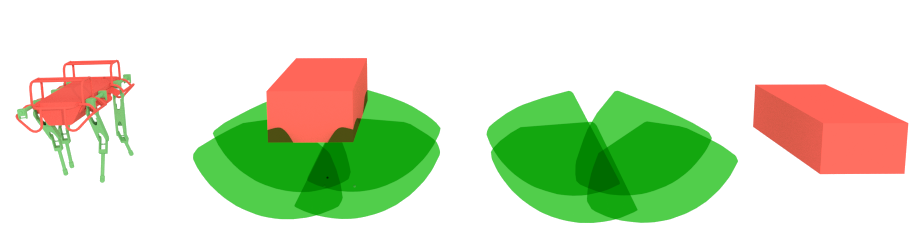
\includegraphics[width=1\linewidth]{figures/HyQ_roms}
  \caption{
           Reachable workspace and torso bounding box of HyQ. Each green shape represent a reachable workspace $W^k$ of a limb. The red shape is $W^0$.}
		   \label{fig:HyQ_roms}
\end{figure}
\section{Root path planning in the contact reachable space}
\label{rbprm}

During the root path planning we only consider the root configuration $\mathbf{q}^0$ defined in the previous Section,
as well as the environment $O$.

Given start and goal configurations, we aim at computing a guide path $\mathbf{q}^0(t) : [0,1] \longrightarrow$ $\mathbb{R}^r$ verifying:
\begin{equation*} \label{eq:path}
\forall t \in [0,1], \mathbf{q}^0(t)  \in C_{Equil}^0
\end{equation*}
This means that any root configuration must be extended into a whole-body, static equilibrium configuration.
$C_{Equil}^0$  cannot be described analytically.

The main hypothesis of this work is that for a large variety of locomotion tasks, we can define a space  $C_{Reach}^0 \simeq C_{Contact}^0$, such that 
\begin{equation} \label{eq:creach}
\forall t \in [0,1], \mathbf{q}^0(t) \in C_{Reach}^0 \Rightarrow \mathbf{q}^0(t)  \in C_{Equil}^0
\end{equation}
We call  $C_{Reach}^0$ the \textit{contact reachable workspace}, and detail its construction in the following.
The validity of this hypothesis is discussed in depth in Section~\ref{sec:discussion}.

\subsection{Conditions for contact reachability}
The contact reachable workspace is defined as a compromise between two necessary and a sufficient condition for contact creation.

\textbf{necessary conditions:}
For a contact to be possible, an obstacle $O_i \subset O$ necessarily intersects the reachable workspace $W(\mathbf{q}^{0})$ of the robot. %
 Also the torso of the robot $W^0(\mathbf{q}^{0})$ must necessarily be collision-free.
Therefore we can define an outer approximation  $ \mathcal{C}^0_{\textrm{\it Nec}} \supset$ $C_{Contact}^0$ as: 
\begin{equation}
\mathcal{C}^0_{\textrm{\it Nec}} = \{ \mathbf{q}^0 : W(\mathbf{q}^{0}) \cap O \neq \emptyset \textrm{ \textbf{and}}\ W^0(\mathbf{q}^{0}) \cap O = \emptyset \} %
\end{equation}

\textbf{sufficient condition:}
Similarly we can define an inner approximation \mbox{$\mathcal{C}^0_{\textrm{\it Suf}} \subset $ $C_{Contact}^0$} by considering a bounding volume $B^{\textrm{\it Suf}}$ encompassing the whole robot in a given pose, except for the effector surfaces. 
\begin{equation}
\mathcal{C}^0_{\textrm{\it Suf}} = \{ \mathbf{q}^0 : W(\mathbf{q}^{0}) \cap O \neq \emptyset \textrm{ \textbf{and}}\ B^{\textrm{\it Suf}}(\mathbf{q}^{0}) \cap O = \emptyset \} %
\end{equation}

\subsection{The compromising reachability condition}
\label{sec:scaling}
The ideal shape $B^*, W^0 \subset B^* \subset B^{\textrm{\it Suf}}$ would define a necessary \textbf{and} sufficient condition for contact creation. 
It would guarantee that any root configuration $\mathbf{q}^{0} \in B^*$ would result in a contact configuration, while any $\mathbf{q}^{0} \notin B^*$ could not.
To our knowledge  $B^*$ has no explicit definition.
Therefore, we approximate $B^*$ to define the contact reachable space $C_{Reach}^0$.

We define $W^0_s$ as the volume $W^0$ subject to a scaling transformation by a factor $s \in \mathbb{R}^+$.
We then consider the spaces $C_{s}^0$
 \begin{equation}
 \label{eq:reachc}
C^0_s = \{ \mathbf{q}^0 : W(\mathbf{q}^{0}) \cap O \neq \emptyset \textrm{ \textbf{and}}\ W^0_s(\mathbf{q}^{0}) \cap O = \emptyset \} %
\end{equation}
The parametrization of $s$ defines a trade-off:
If $s=1$, then $W^0_s$ = $W^0$, such that $C_1^0$ = $\mathcal{C}^0_{\textrm{\it Nec}}$.
By increasing $s$, the condition can become sufficient, but less and less necessary.  
Eq.~\ref{eq:reachc} thus defines the \textit{reachability condition}. We fix a value $s^*$ for $s$ and define  $C_{Reach}^0 = C^0_{s^*}$.
The computation of $s^*$ is detailed in Section~\ref{sec:params}. 
In Appendix~\ref{app:rom}, we give a generic method to compute the $W$ volumes appearing in the definition of $C_{Reach}^0$.

\subsection{Computing the guide path in $C_{reach}^0$}
$C_{Reach}^0$ can be sampled efficiently thanks to Eq.~\ref{eq:reachc}, and can thus be used with any standard motion planner.
Our current implementation uses the Bi-RRT planner \citep{770022} provided by the HPP software~\citep{7759083}.
Our implementation is exactly the same as the pseudo-code of the original planner (which does not detail the configuration validation method). With respect to a ``classic'' implementation, the only difference is that instead of validating a configuration using collision detection, we validate it with the \textit{reachability condition}.\\

This Section has presented a guide path planner for the geometric root of a robot, implemented as a low-dimensional sampling-based 
algorithm. Given start and goal configurations, it outputs a continuous path for the robot's root. 
\section{From a guide path to a discrete sequence of contact configurations ($\mathcal{P}_2$)}
\label{sec:contact}
In the second phase, we compute a discrete sequence of static equilibrium configurations $\mathbf{Q}^{\overline{0}}$ given a root path
$\mathbf{q}^0(t) : [0,1] \longrightarrow$ \gls{$C_{Reach}^0$}. This contact planner uses a contact generator, used to generate static equilibrium configurations. We first describe the contact planning algorithm, before describing
the contact generator.

\subsection{Definition of a contact sequence}
In previous contributions~\citep{DBLP:conf/iser/EscandeKMG08}, a contact plan is defined as a sequence of quasi-static equilibrium configurations
for each contact phase. For instance, a walk cycle would be described by three key configurations: a double-support configuration, a single-support configuration (a contact is broken), and another double-support configuration (a contact is created). 
Our definition of contact plan differs: between two consecutive configurations we allow both a contact break and a contact creation---if they are on the same effector. 
In the previous example, our contact plan would simply consist of the two double-support configurations. 
This representation is sufficient to describe all the contact phases, because the single support phase is implicitly described. Furthermore it removes the need to compute a single-support quasi-static configuration as in the example. Indeed, there might be a case where no quasi-static solution exists for the single support phase (because of the environment), but
there exists a dynamic motion connecting the two double support states. Such motion will be computed by our framework, because the quasi-static constraint is only required at the contact planning phase; as shown in the companion video, and explained in Appendix~\ref{app:optim}, our framework is able to produce dynamic motions.

\subsection{Contact planning algorithm}
Starting from an initial whole-body configuration, we compute a sequence
of whole-body configurations  $\mathbf{Q}^{\overline{0}}$ along the root path $\mathbf{q}^0(t)$.
We first give an intuition of the algorithm, before providing its complete pseudo-code.
\subsubsection{Algorithm overview}
First, the root path $\mathbf{q}^0(t)$ is discretized into a sequence of $j$ key configurations:  
\begin{equation*}
	\mathbf{Q}^0 = [\mathbf{q}^0_{0}; \mathbf{q}^0_{i}; ..., \mathbf{q}^0_{j-1}]
\end{equation*} 

where $\mathbf{q}^0_{0}$ and $\mathbf{q}^0_{j-1}$ are the start and goal configurations. %
$j$ depends on a user-defined variable, called the discretization step. It corresponds to the ratio between the length of the path $\mathbf{q}^0(t)$\footnote{The length of the path is computed as the weighted 6D Euclidean distance
traveled along the it, with a weight of $0.7$ for the translation part, and $0.3$ for the orientation part.}, and the number
of configurations selected along it to create the contact configurations. 
Each root configuration of $\mathbf{Q}^0$ is then extended into a whole-body configuration such that:
\begin{itemize} 
\item At most one contact is not maintained (\textit{broken}) between two consecutive configurations.
\item At most one contact is added between two consecutive configurations.
\item Each configuration is in static equilibrium.
\item Each configuration is collision-free.
\end{itemize} 

\paragraph{Maintaining a contact in the sequence}

If kinematically possible, a limb in contact at step $i-1$ remains in contact at step $i$ (Figure~\ref{fig:break_contact}). 
Otherwise the contact is broken and a collision-free configuration is assigned to the limb.
If two or more contacts can't be maintained between two consecutive configurations, one or more intermediate configurations are added, to ensure
that at most one contact is broken between two sequential configurations.

\begin{figure}[t]
\centering
  \begin{overpic}[width=1\linewidth]{figures/break_contact}
		\put (0,4) {1} 
		\put (25,4) {2} 
		\put (50,4) {3} 
		\put (76,4) {4} 
	\end{overpic}
\caption{Contacts are maintained if joint limits and collisions constraints are respected (2). They are broken otherwise(3,4). The green line represents the root path. The blurred character
represents the previous contact configuration.}
		   \label{fig:break_contact}
\end{figure}

\paragraph{Creating contacts}
Contacts are created using a FIFO approach: we try first to create a contact with the limb that has been contact-free the longest. If the contact creation does not succeeds, the limb is pushed on top of the queue, and will only be tried again after the others. \\ \\

\subsubsection{Pseudo-code of the Algorithm}
\label{app:contact}

From the start configuration, given as an input by the user,
we create the initial state $s0$. A state is described by a whole-body configuration, as well as the list of currently active contacts and their associated 6D positions.
Algorithm~\ref{alg:interpolate}  is then called with $s0$, as well as the discretized path 
$\mathbf{Q}^0$, as input parameters.

\begin{algorithm}[!tbp]
\caption{Discretization of a path} \label{interpolate}
	\begin{algorithmic}[1]
	\Function{Interpolate}{$s0$,$\mathbf{Q}^0$, $MAX\_TRIES$}
		\State $states \gets (s0)$ \Comment{List of states initialized with $s0$}
		\State $nb\_fail \gets 0$ 
		\State $i \gets 1;$ \Comment{Current index in the list}
		\While {$i < Length(\mathbf{Q}^0)$}
			\State $pState \gets LastElement(states)$
			\State $s \gets$ \textsc{GenFullBody}$(pState, Element(\mathbf{Q}^0,i))$
			\If {$s \not= 0 $}
				\State $nb\_fail \gets 0$
				\State $i \gets i+1$
			\Else
				\State $nb\_fail \gets nb\_fail + 1$
				\State $s \gets $\textsc{IntermediateContactState}$(pState)$
				\If {$s == 0 \lor nb\_fail == MAX\_TRIES$}
					\State \textbf{return} $FAILURE$
				\EndIf		
			\EndIf
			\State ${PushBack}(states, s)$
		\EndWhile
		\State \textbf{return} $states$
	\EndFunction
\end{algorithmic}
\label{alg:interpolate}
\end{algorithm}

At each step of Algorithm~1, \textsc{GenFullBody} (Algorithm~\ref{alg:pi}) is called with the previous state as a parameter, as well
as a new root configuration. \textsc{GenFullBody} returns a new contact configuration, if it succeeded
in computing a configuration with only one contact switch occurring~;
otherwise, the method \textsc{IntermediateContactState} (Algorithm~\ref{alg:repo}) is called.
It repositions an end effector (either a free limb, or the oldest active contact) towards a new contact position if possible.
This repositioning allows to increase the odds that the contact can be maintained at the next step.
The method \textit{Length} returns the length of a list~; \textit{LastElement} returns the last element
of a list~; \textit{Element} returns the element of a list at a given index~; and \textit{PushBack} inserts an element at the end of a list.

\begin{algorithm}[!tbp]
\caption{Full body contact generation method} \label{interpolate}
	\begin{algorithmic}[1]
	\Function{\textsc{GenFullBody}}{$pState$,$\mathbf{q}^0$}
		\State $newState \gets {CreateState}(\mathbf{q}^0,$ 
        \State $\quad \quad \quad \quad  \quad  \quad  \quad  \quad  \quad \quad  \quad \quad\!\! ContactLimbs(pState))$
		\State $nConBroken \gets 0$
		\For {\textbf{each} $k$ in $ContactLimbs(pState)$}
			\If {$\neg$\textit{MaintainContact}$(pState,\mathbf{q}^0,k)$}
				\State $nConBroken \gets nConBroken +1$
				\If {$nConBroken > 1$}				
					\State \textbf{return} $0$
				\EndIf				
				\State \textit{MarkFree}$(newState,k)$
			\Else 					
				\State \textit{MarkContact}$(newState,k)$
			\EndIf
		\EndFor
		\For {\textbf{each} $k$ in $FreeLimbs(newState)$}
			\If {\textit{GenerateContact}$(newState,k)$}	
				\State \textit{MarkContact}$(newState,k)$
				\State \textbf{return} $newState$
			\EndIf
		\EndFor
		\If {\textit{IsInStaticEquilibrium}$(newState)$}
			\State \textbf{return} $newState$
		\Else
			\State \textbf{return} $0$
		\EndIf
	\EndFunction
\end{algorithmic}
\label{alg:pi}
\end{algorithm}

In Alg.~\ref{alg:pi}, the procedure \textit{MaintainContact}$(pState,\mathbf{q}^0,k)$ performs inverse kinematics to reach the previous contact position for the limb.
If it succeeds, the new limb configuration is assigned to $k$. If it fails, a random collision free configuration is assigned to $k$.
The method \textit{IsInStaticEquilibrium} returns whether a given state is in static equilibrium. \textit{CreateState} creates a new state, given
a root configuration and the list of active contacts.
$ContactLimbs$ (respectively $FreeLimbs$) returns the list of limbs that are in contact (respectively \textit{not} in contact).  \textit{MarkContact} (respectively \textit{MarkFree})  marks a limb as in contact (respectively \textit{not} in contact). These methods follow a FIFO approach: the first limb chronologically marked as in contact (respectively not in contact) is returned first by $ContactLimbs$ (respectively $FreeLimbs$). This allows the algorithm to be deterministic even though it can handle acyclic motions.
\textit{GenerateContact}$(state,k)$ is a call to the contact generator presented in the following Section~\ref{sec:single_contact}.
It generates a contact configuration in static equilibrium, and assigns the corresponding configuration of the limb $k$ to the state configuration.
If it fails, $k$ remains unchanged if collision free, else it is assigned a random collision free configuration.

Algorithm~\ref{alg:repo} generates an intermediate state by first trying to create a contact with one of the free limbs (trying in a FIFO order) then by repositioning one of the limbs in contact.

\begin{algorithm}[!tbp]
\caption{Adds or repositions a contact for one limb} \label{interpolate}
	\begin{algorithmic}[1]
	\Function{IntermediateContactState}{$state$}        
        \State $newState \gets state$
		\For {\textbf{each} $k$ in $FreeLimbs(newState)$}
			\If {\textit{GenerateContact}$(newState,k)$}	
				\State \textit{MarkContact}$(newState,k)$			
				\State \textbf{return} $newState$
			\EndIf
		\EndFor
		\For {\textbf{each} $k$ in $ContactLimbs(newState)$}
			\If {\textit{GenerateContact}$(newState,k)$}	
				\State /*Account for repositioning in FIFO queue*/		
				\State \textit{MarkContact}$(newState,k)$
				\State \textbf{return} $newState$
			\EndIf
		\EndFor
        \State
		/*Fails if impossible to relocate any effector*/
		\State \textbf{return} $0$
	\EndFunction
\end{algorithmic}
\label{alg:repo}
\end{algorithm}

\subsection{Contact generator}
\label{sec:single_contact}

\begin{figure*}
  \centering
  \begin{overpic}[width=0.8\linewidth]{figures/contact_gen}
		\put (1,1) {a} 
		\put (22,1) {b} 
		\put (42,1) {c} 
		\put (62,1) {d} 
		\put (83,1) {e} 
	\end{overpic}
  \caption{Generation of a contact configuration for the right leg of HRP-2. (a): Selection of reachable obstacles. (b): Entries of the limb samples database (with $N = 4$). (c): With a proximity query between the octree database and the obstacles, configurations too far from obstacles are discarded. (d): The best candidate according to a user-defined heuristic $h$ is chosen. (e): The final contact is achieved using inverse kinematics.}
  \label{fig:contact_gen}
\end{figure*}

Given a configuration of the root and the list of effectors that should be in contact, the contact generator computes the configuration of the limbs such that contacts are properly satisfied and the robot is in static equilibrium:

\begin{equation}
\label{eq:contact_gen}
	\mathbf{q}^{\overline{k}}  \longrightarrow \mathbf{q}^k, (\mathbf{q}^{k} \oplus \mathbf{q}^{\overline{k}}) \in  C_{Equil} \textrm{ \textbf{and}}\ \mathbf{q}^k \in  C_{Contact}^k 
\end{equation}

In previous works~\cite{DBLP:conf/iser/EscandeKMG08,Bouyarmane2009}, the generation of contact is typically implemented by randomly sampling configurations and projecting the whole robot configuration onto the closest surfaces with an inverse kinematics solver.
In case of failure of the projection, the process would randomly iterate.

We propose two modifications of this general algorithm principle.
First our contact generator handles each limb $R^k$ independently.
By handling each limb separately, we reduce the complexity of the generation of contact configurations.
This is made possible thanks to the reachability condition in $\mathcal{P}_1$ that produces a root path that we can afford not to modify in $\mathcal{P}_2$, and because we allow both a contact break and a contact creation between two consecutive configurations of the contact sequence.
Second, we rely on off-line generation of configuration candidates.

We define $C_{Contact}^{\epsilon} \supset C_{Contact}$ as the set of configurations such that the minimum 3D distance 
between an effector and an obstacle is less than $\epsilon \in \mathbb{R}$.
We then apply the following steps:
\begin{enumerate}
\item Generate off-line $N$ valid sample limb configurations $\mathbf{q}^k_i,  0 \leq i < N$ (We choose $N=10^4$);
\item Using the end-effector positions $\mathbf{p}(\mathbf{q}^k_i)$ as indices, store each sample in an octree data structure;
\item At runtime, when contact creation is required, intersect the octree and the environment to retrieve the list of samples $S \subset C_{Contact}^{\epsilon}$ close to contact (Figure~\ref{fig:contact_gen} (b) and (c)). This operation is achieved natively by the fcl library \cite{6225337};
\item Use a user-defined heuristic $h$ to sort $S$;
\item If $S$ is empty, stop (failure). Else select the first configuration of $S$. Project it onto contact using inverse kinematics. (Figure~\ref{fig:contact_gen} (d) and (e));
\item If Eq.~\ref{eq:contact_gen} is verified, stop (success). Otherwise remove the element from $S$ and go to step 5.
\end{enumerate}

Because the distance $\epsilon$ does not account for the variation in orientation, several samples of $ C_{Contact}^{\epsilon}$  may turn out to be unfeasible at the time of projection. One could consider additionally filtering $ C_{Contact}^{\epsilon}$ based on the orientation with respect to the obstacle normal, but in our experience we did not notice
any significant improvement in the computational performances of the planner, so we do not perform this additional step. 

In all our experiments, the heuristic $h$ is implemented as a variation of a manipulability-based heuristic~\cite{Yoshikawa1984}. The manipulability is a real number that quantifies how 
``good'' a configuration is to perform a given task, based on the analysis of the Jacobian matrix. With such heuristics, a configuration can be chosen because it is far from singularities, and thus allows mobility in all directions. On the contrary, it can be chosen because it is particularly efficient to exert a force in a desired direction. In our experiments, the former solution is usually chosen for computing leg contacts, while the latter is used for computing hand contacts. We recall the manipulability measure and its derivatives in Appendix~\ref{sec:heuristics}.

Finally, to verify that a configuration is in static equilibrium, we use a new robust LP formulation. It replaces the computationally inefficient double description
approach used in our previous work~\cite{tonneauisrr15}, and presented in the following Section~\ref{sec:Equil}.

\section{A criterion for robust static equilibrium}
\label{sec:Equil}

We first give a linear program (LP) that verifies whether a contact configuration allows for static equilibrium. This LP is the same that was proposed in  \citep{Prete2016}.
From this formulation we derive a new LP that quantifies the robustness of the equilibrium to uncertainties in the contact forces.
In turn, from this value we can either choose the most robust candidate, or set a threshold on the required robustness. 

\subsubsection{Conditions for static equilibrium}
We first define the variables of the problem, for $e$ contact points, expressed in world coordinates:
\begin{itemize}
\item $\mathbf{c} \in \mathbb{R}^3$ is the robot center of mass (COM);
\item $m \in \mathbb{R}$ is the robot mass;
\item $\mathbf{g} = [0,0,-9.81]^T$ is the gravity acceleration;
\item $\mu$ is the friction coefficient;
\item for the i-th contact point $1 \leq i \leq e$:
	\begin{itemize}
	\item $\mathbf{p_i}$ is the contact position;
	\item $\mathbf{f_i}$ is the force applied at $\mathbf{p_i}$;
	\item $\mathbf{n}_i,\mathbf{\boldsymbol\upgamma}_{i1},\mathbf{\boldsymbol\upgamma}_{i2}$ form a local Cartesian coordinate system centered at $\mathbf{p_i}$. $\mathbf{n}_i$ is aligned
	with the contact surface normal, and the $\mathbf{\boldsymbol\upgamma}_i$s are tangent vectors.
	\end{itemize}
\end{itemize}

According to Coulomb's law, the non-slipping condition is verified if all the contact forces lie in the friction cone defined by the surface.
Classically, we linearize the friction cone in a conservative fashion with a pyramid included in it, described by four generating rays of unit length. We choose for instance:
\begin{equation*}
\mathbf{V}_{i} = \mat{\mathbf{n}_{i} + \mu \mathbf{\boldsymbol\upgamma}_{i1} & \mathbf{n}_{i} -\mu \mathbf{\boldsymbol\upgamma}_{i1} & \mathbf{n}_{i} + \mu \mathbf{\boldsymbol\upgamma}_{i2} & \mathbf{n}_{i} - \mu \mathbf{\boldsymbol\upgamma}_{i2}}^T
\end{equation*}

Any force belonging to the linearized cone
can thus be expressed as a positive combination of its four generating rays.

\begin{equation*}
\forall i  \qquad  \exists \bm{\beta}_i \in \mathbb{R}^{4} : \bm{\beta}_i \ge 0 \text{ and } \mathbf{f}_{i} = \mathbf{V}_{i} \bm{\beta}_i,
\end{equation*}
where $\bm{\beta}_i$ contains the coefficients of the cone generators.
We can then stack all the constraints to obtain:
\begin{equation}\label{eq:gen}
\exists \bm{\beta} \in \mathbb{R}^{4e} ,  \bm{\beta} \ge 0 \text{ and } \mathbf{f} = \mathbf{V} \bm{\beta},
\end{equation}
where $\mathbf{V} = \diag{ \{\mathbf{V}_1, \dots, \mathbf{V}_e\} }$, and $\mathbf{f} = (\mathbf{f}_0,...,\mathbf{f}_e)$.

From the Newton-Euler equations, to be in static equilibrium the contact forces have to compensate the gravity:

\begin{align} \label{eq:new_eul}
\underbrace{
\mat{\mathbf{I}_3 & \dots & \mathbf{I}_3 \\
\hat{\mathbf{p}}_1 & \dots & \hat{\mathbf{p}}_e} \mathbf{V}
}_\mathbf{G} \bm{\beta}, = 
\underbrace{\mat{\mathbf{0}_{3\times 3} \\ m \hat{\mathbf{g}}}}_{\mathbf{D}} \mathbf{c} + 
\underbrace{\mat{-m\mathbf{g} \\ \mathbf{0}}}_{\mathbf{d}}
\end{align}
where $\hat{\mathbf{x}} \in \R{3}{3}$ is the cross-product matrix associated to $\mathbf{x}$.

If there exists a $\bm{\beta}^*$ satisfying \eqref{eq:gen} and \eqref{eq:new_eul}, it means that the configuration is in static equilibrium.
The problem can then be formulated as an LP:

\begin{equation} \label{eq:lin_prog} \begin{aligned}
\find \quad & \bm{\beta} \in \Rv{4e} \\
\st \quad &\mathbf{G} \bm{\beta} = \mathbf{D} \mathbf{c} + \mathbf{d} \\
& \bm{\beta} \ge 0 \\
\end{aligned} \end{equation}

\subsubsection{Formulation of a robust LP}
Let $b_0 \in \mathbb{R}$ be a scalar value. We now define the following LP:

\begin{equation} \label{eq:lin_prog_rob} \begin{aligned}
\find \quad & \bm{\beta} \in \Rv{4e}, b_0 \in \Rv{} \\
\minimize  \quad & -b_0 \\
\st \quad &\mathbf{G} \bm{\beta} = \mathbf{D} \mathbf{c} + \mathbf{d} \\
& \bm{\beta} \ge b_0 \bm{1}\\
\end{aligned} \end{equation}

We observe that if $b_0$ is positive then \eqref{eq:lin_prog} admits a solution, and $b_0$ is proportional to the minimum distance of the contact forces to the boundaries of the friction cones.
If $b_0$ is negative, the configuration is not in static equilibrium, and $b_0$ indicates ``how far'' from equilibrium the configuration is. We thus use $b_0$ as a measure of robustness.
A simple approach to robustness consists in choosing a smaller friction coefficient, to constrain the forces to lie away from the boundaries of the real cone.  However, this would result in a small safety margin for forces of low magnitude, and an excessively large safety margin for large forces as the boundaries grow more and more apart. In comparison, our margin $b_0$ is constant, and provides a helpful mean to compare the robustness of different contact configurations.

In our implementation, rather than solving directly \eqref{eq:lin_prog_rob}, we solve an equivalent problem of smaller dimension that we get by taking the dual of \eqref{eq:lin_prog_rob} and eliminating the Lagrange multipliers associated to the inequality constraints:
\begin{equation} \label{eq:dual} \begin{aligned}
\find \quad & \bm{\nu} \in \Rv{6}\\
\maximize  \quad & -(\mathbf{D} \mathbf{c} + \mathbf{d})^T \bm{\nu} \\
\st \quad &\mathbf{G}^T \bm{\nu} \ge 0 \\
& \mathbf{1}^T \mathbf{G}^T \bm{\nu} = 1 \\
\end{aligned} \end{equation}

The optimal value $\bm{\nu}^*$ gives the optimal value $b_0^*$ through the equality $b_0^* = (\mathbf{D} \mathbf{c} + \mathbf{d})^T \bm{\nu}^*$.

\section{Source code of our planner}
\label{app:hpp}
Our planner is implemented using the Humanoid Path Planner (HPP) software, introduced in~\cite{7759083}.
HPP is an open source motion planning framework developed by the Gepetto team at LAAS-CNRS.
HPP implements the standard tools and algorithms used in motion planning,
such as the Bi-RRT planner from which RB-RRT is derived.

The robot models used in our experiments are described using the standard urdf file format, compatible with HPP.

Our implementation of the planner is also open source.
Both HPP and our planner can be simply downloaded and compiled by following the instructions on
\url{http://stevetonneau.fr/files/publications/isrr15/tro_install.html}. 
\section{Results}
\label{sec:results}
In this section we present some of the results obtained with our planner. The complete sequences are shown in the companion video.
Specifically, we demonstrate the planner for two legged robots, in a large variety of environments: the humanoid HRP-2 and the quadruped HyQ.

Our contact plans are then interpolated with a dedicated solution to the interpolation problem $\mathcal{P}_3$. This allows us to validate the obtained
motions in a dynamic simulator. This validation is an important contribution as it increases the confidence that the contact plans we compute can effectively
result in feasible motions on the real robot. One motion is demonstrated on the real HRP-2 robot.

At the end of this section, we discuss the role of the parameters of our framework. We then provide the \textit{interactive} computation times obtained in each case.
We also compare the times obtained with HRP-2 with respect to previous works.

\subsection{Experimental validation of the contact plans} \label{sec:valid}
To generate continuous movements from our contact plans we used either the framework proposed in \cite{Carpentier2016}, or our own implementation of a $\mathcal{P}_3$ solver (Appendix~\ref{app:optim}).
The resulting movements have been validated either on the real HRP-2 robot (details can be found in~\cite{Carpentier2016}), or with our dynamic simulator, based on a state-of-the-art algorithm~\cite{Kaufman2008}.
In the simulations we controlled the robot with a standard inverse-dynamics controller~\cite{DelPrete2015b}. The code source of the simulator is available at \url{http://stevetonneau.fr/files/publications/isrr15/tro_install.html\#simulator}.
This controller tries to follow the given whole-body trajectories, giving higher priority to the center-of-mass and end-effectors tracking with respect to the joint tracking.
The controller also makes sure that the resulting contact forces lie inside the specified friction cones (we used a friction coefficient of 0.3), and that the joint position, velocity and torque limits are satisfied.
The companion video shows the obtained motions.

\subsection{Description of the scenarios}
In all the scenarios considered, the formulation of the problem is always the same:
a start and goal root configuration are provided as input (except in the stair climbing scenario where the start whole body configuration is given).
The framework computes the initial contact configuration, and outputs a sequence of contact configurations connecting it to the goal.
In each scenario we detail the contacts involved and the heuristics chosen (either $h_{\textrm{\it EFORT}}$, $h_{vel}$ or $h_{w}$, all of which are defined in the Appendix~\ref{sec:heuristics}).

\subsubsection{HRP-2 -- Standing up (Figure~\ref{fig:standing})}
From a bent configuration, the robot has to stand up using a wall as support, and climbing a 25-cm high step.

\begin{figure}
  \centering
  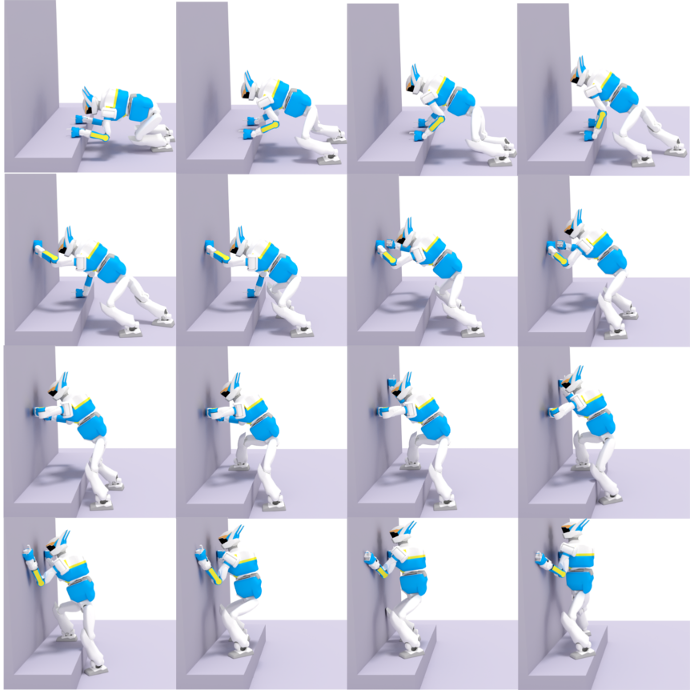
\includegraphics[width=1\linewidth]{figures/standing}
  \caption{
           HRP-2 in the standing scenario. }
		   \label{fig:standing}
\end{figure}

\noindent\textbf{Contacts involved:} All (both feet and hands).

\noindent\textbf{Heuristics:} $h_w$ for the feet, $h_{\textrm{\it EFORT}}$  for the hands.

\subsubsection{HRP-2 -- Car egress (Figure~\ref{fig:car})}
In this scenario inspired from the DRC car egress HRP-2 has to step out of a car.

\begin{figure}
  \centering
  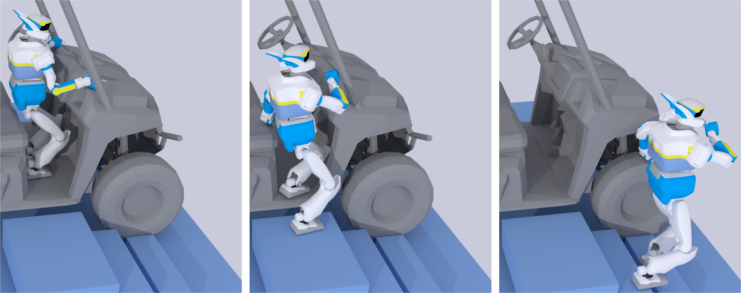
\includegraphics[width=1\linewidth]{figures/polaris}
  \caption{
           Selected frames from the car egress scenario. }
		   \label{fig:car}
\end{figure}

\noindent\textbf{Contacts involved:} All (both feet and hands).

\noindent\textbf{Heuristics:} $h_w$.

\subsubsection{HRP-2 -- Staircase with high steps (Figure~\ref{fig:stair_robust})}
\newcommand{\widthValue}{0.13\linewidth}

\begin{figure*}[h!t!]
  \begin{center}
  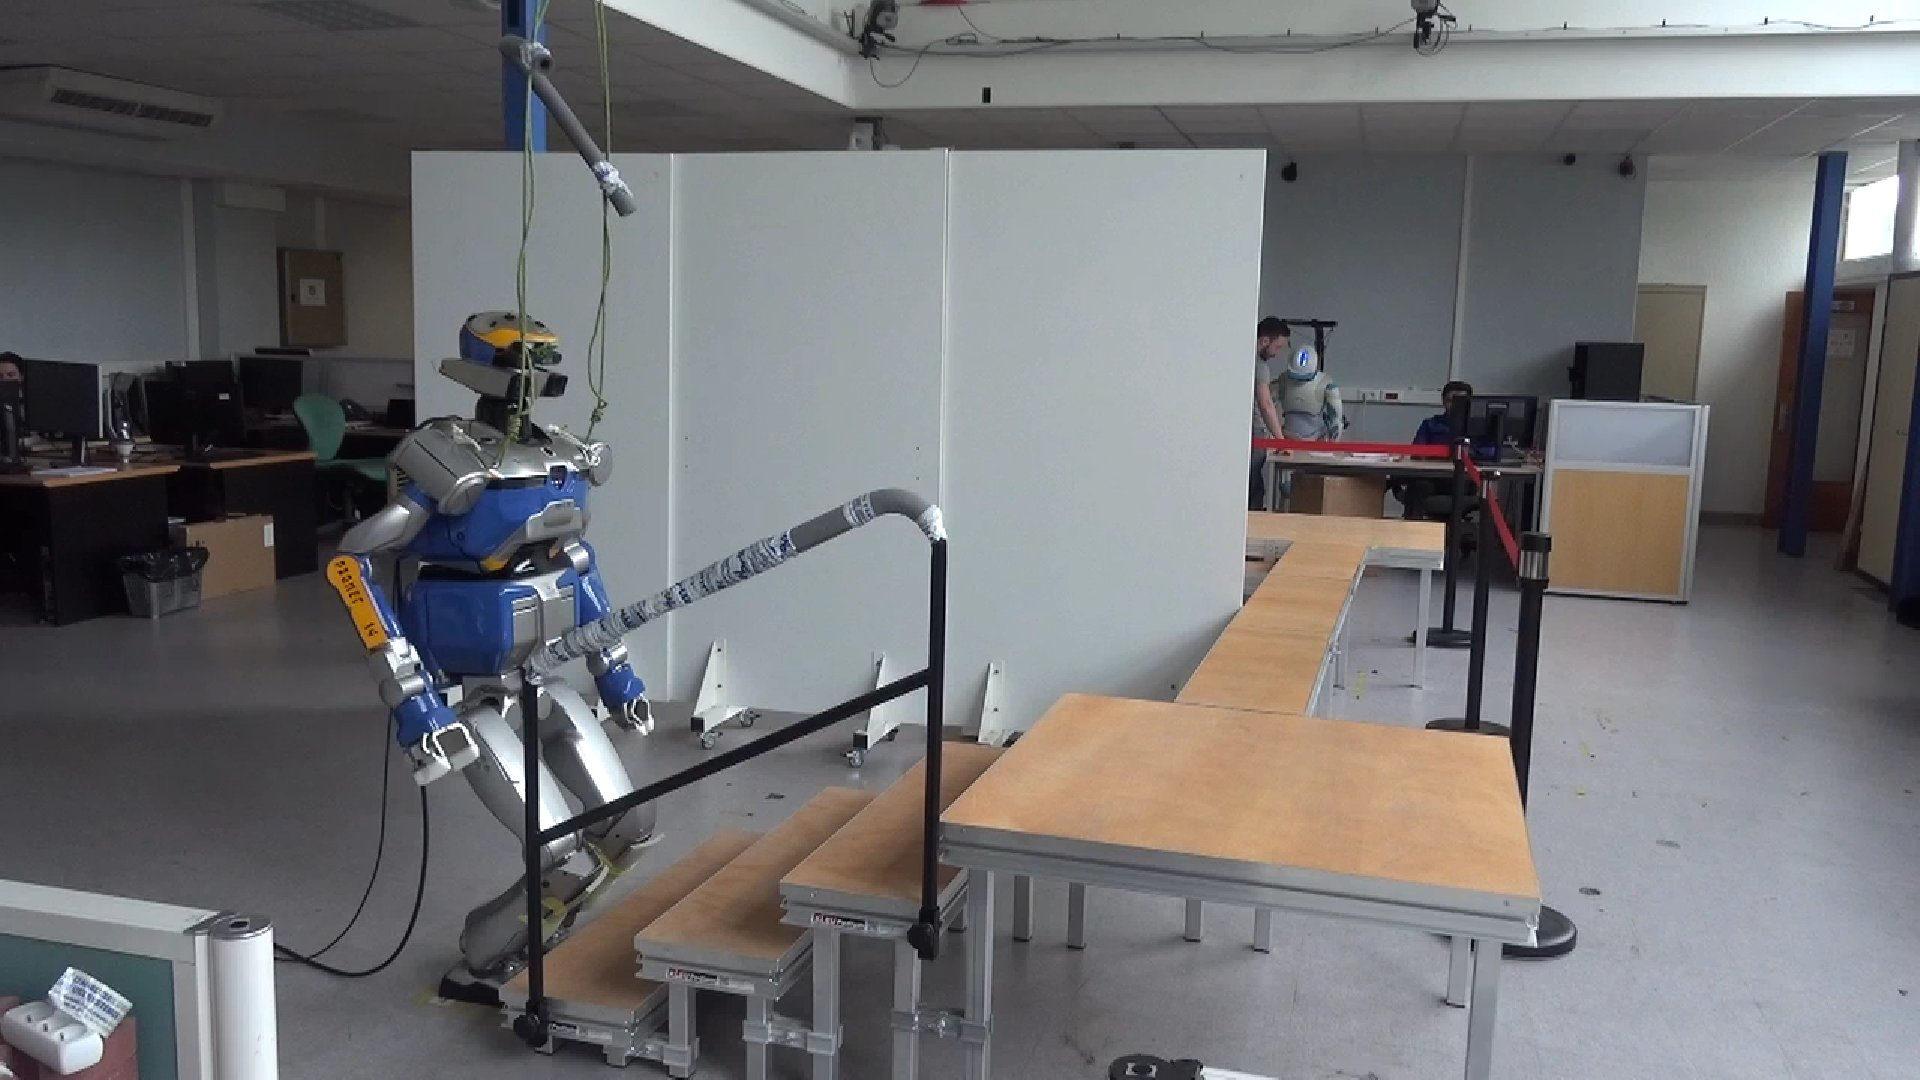
\includegraphics[trim={7.0cm 0.0cm 20.0cm 0.0cm}, clip, width=\widthValue]
    {./figures/stairclimbing1.jpeg}
  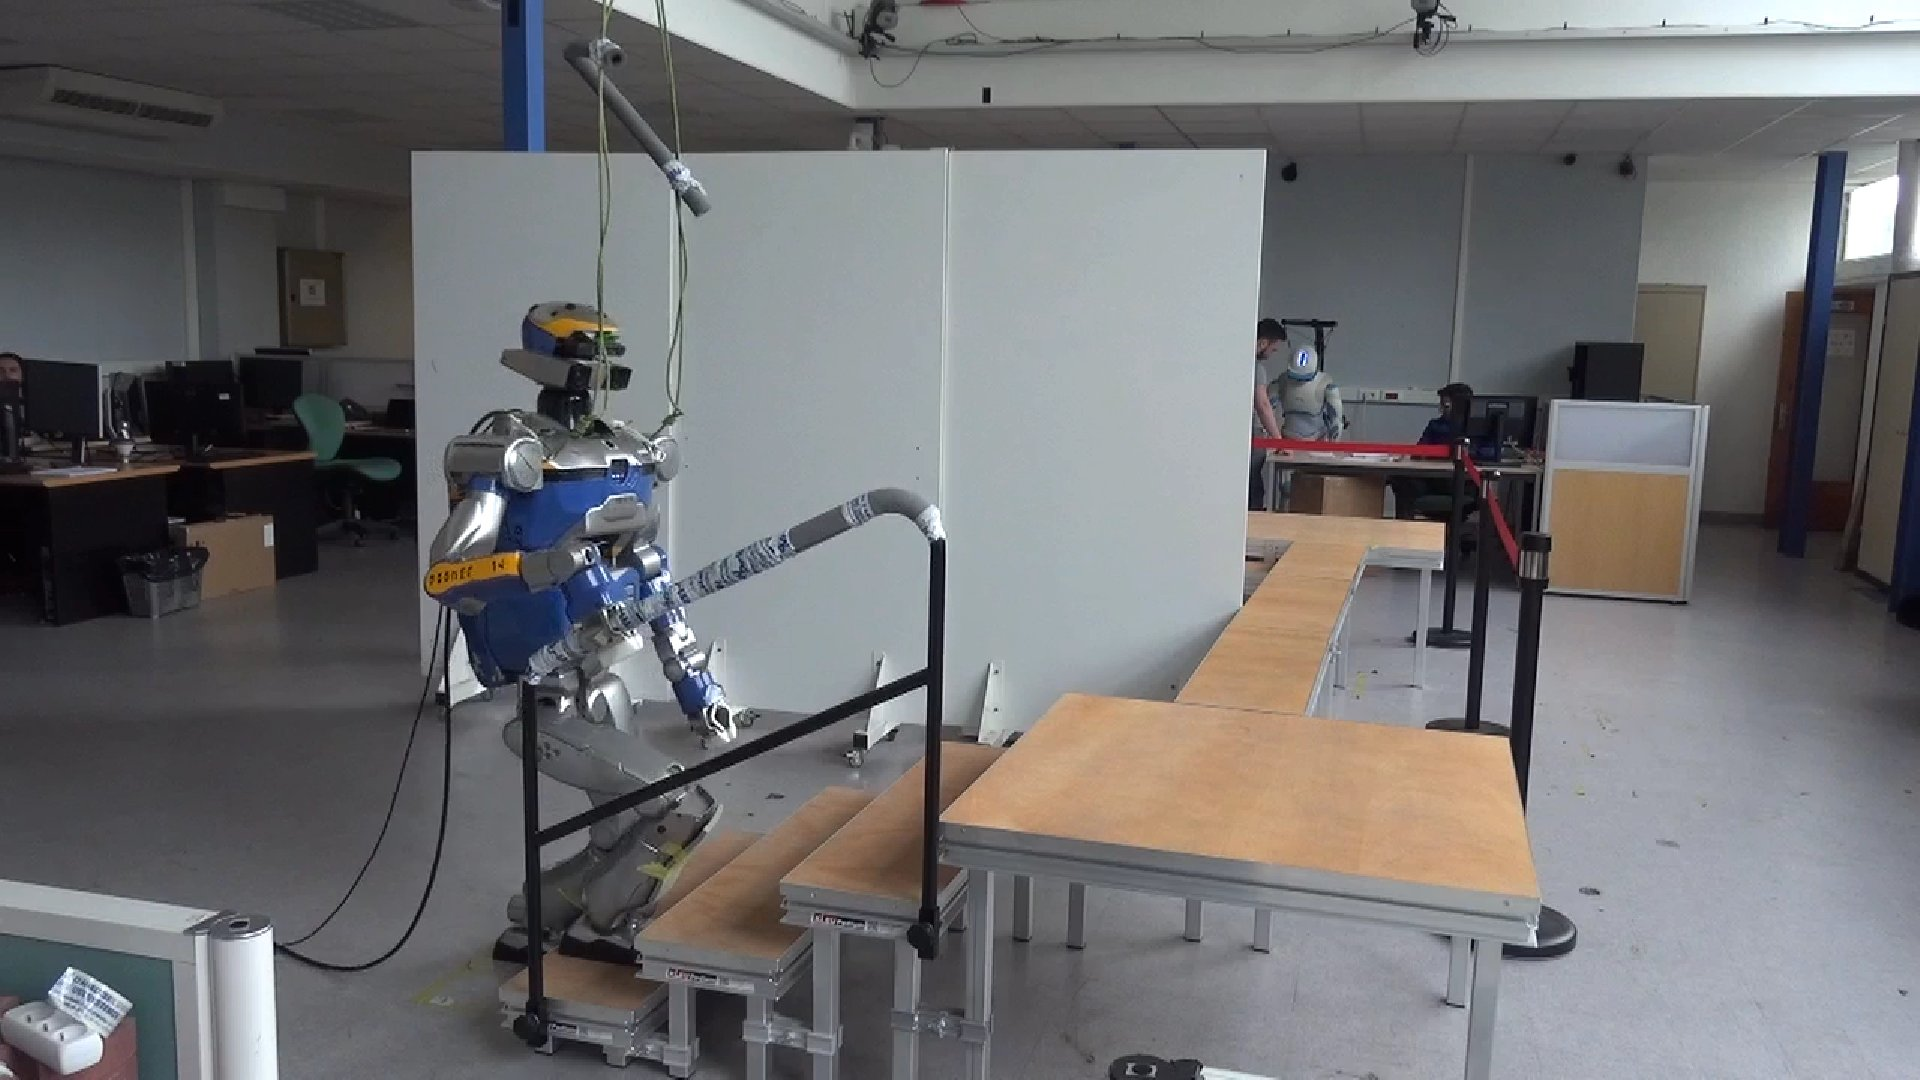
\includegraphics[trim={7.0cm 0.0cm 20.0cm 0.0cm}, clip, width=\widthValue]
    {./figures/stairclimbing2.jpeg}
  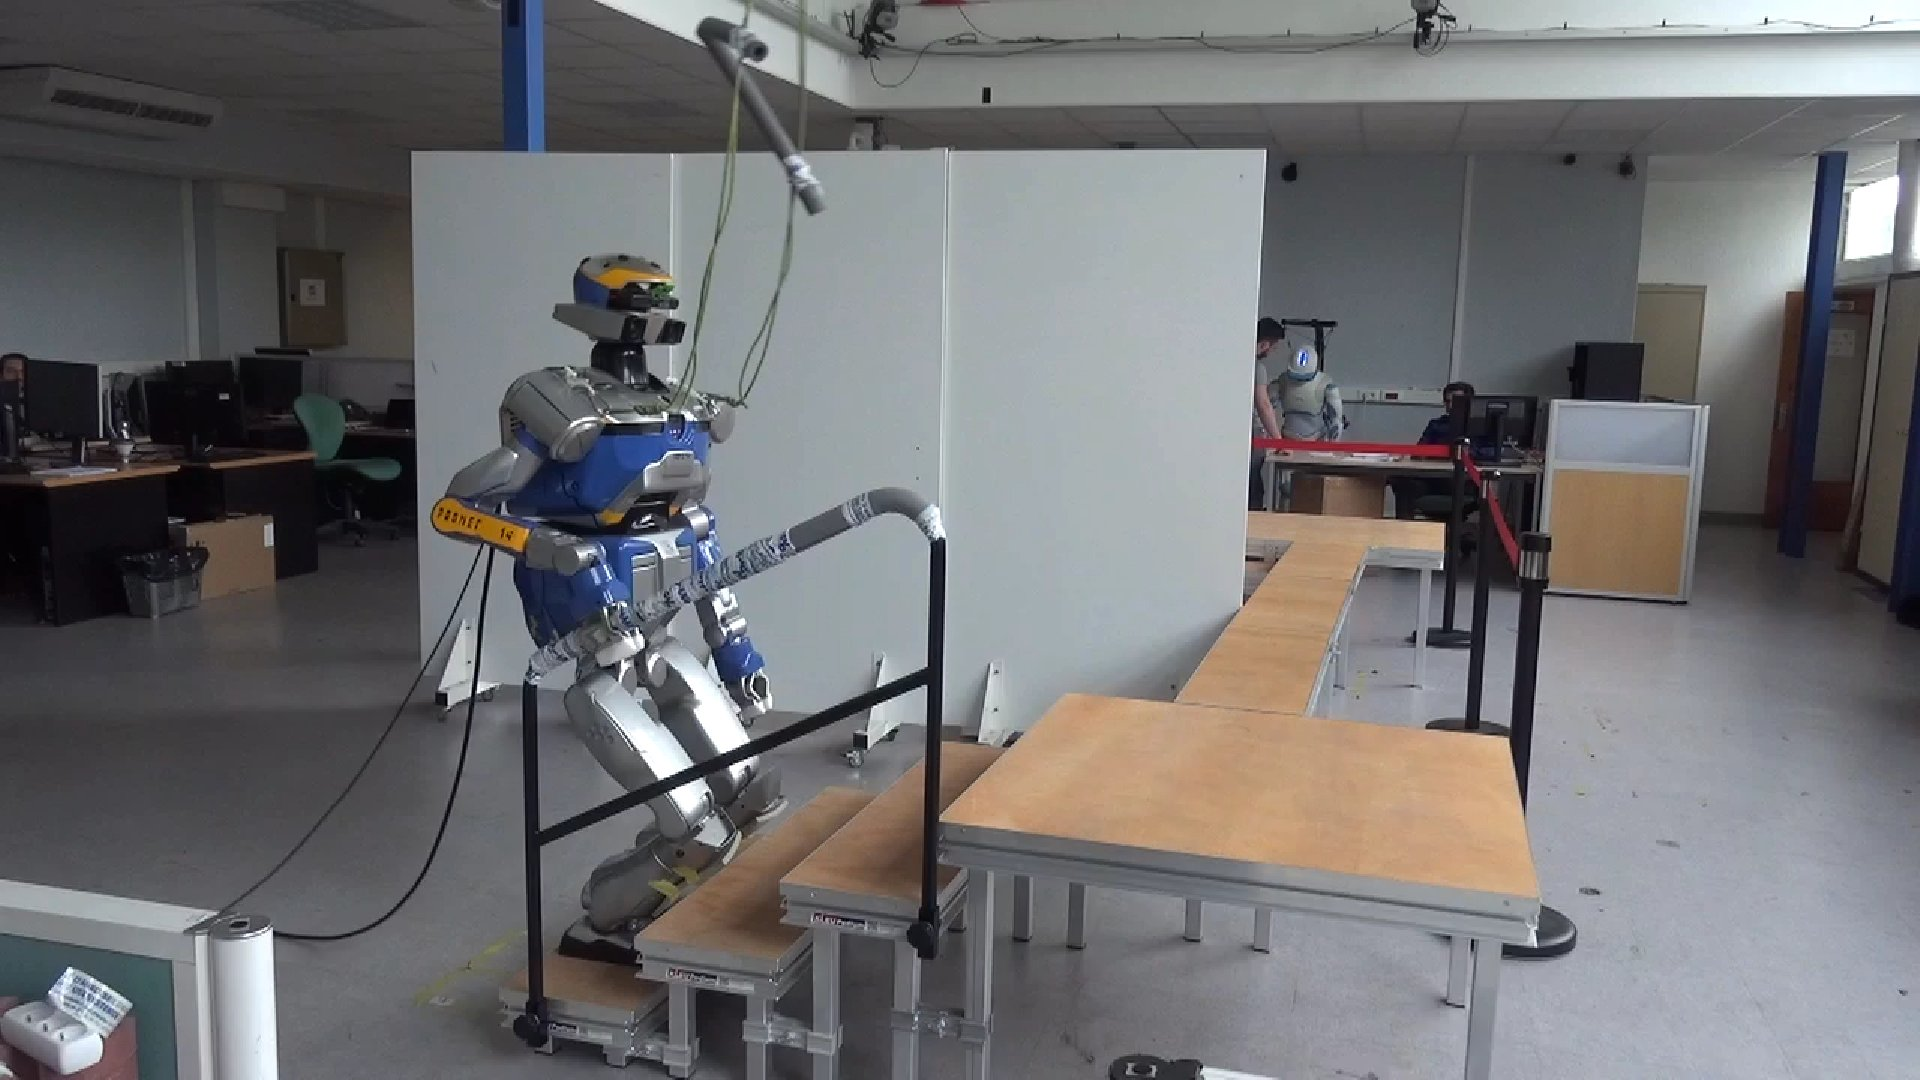
\includegraphics[trim={7.0cm 0.0cm 20.0cm 0.0cm}, clip, width=\widthValue]
    {./figures/stairclimbing3.jpeg}
  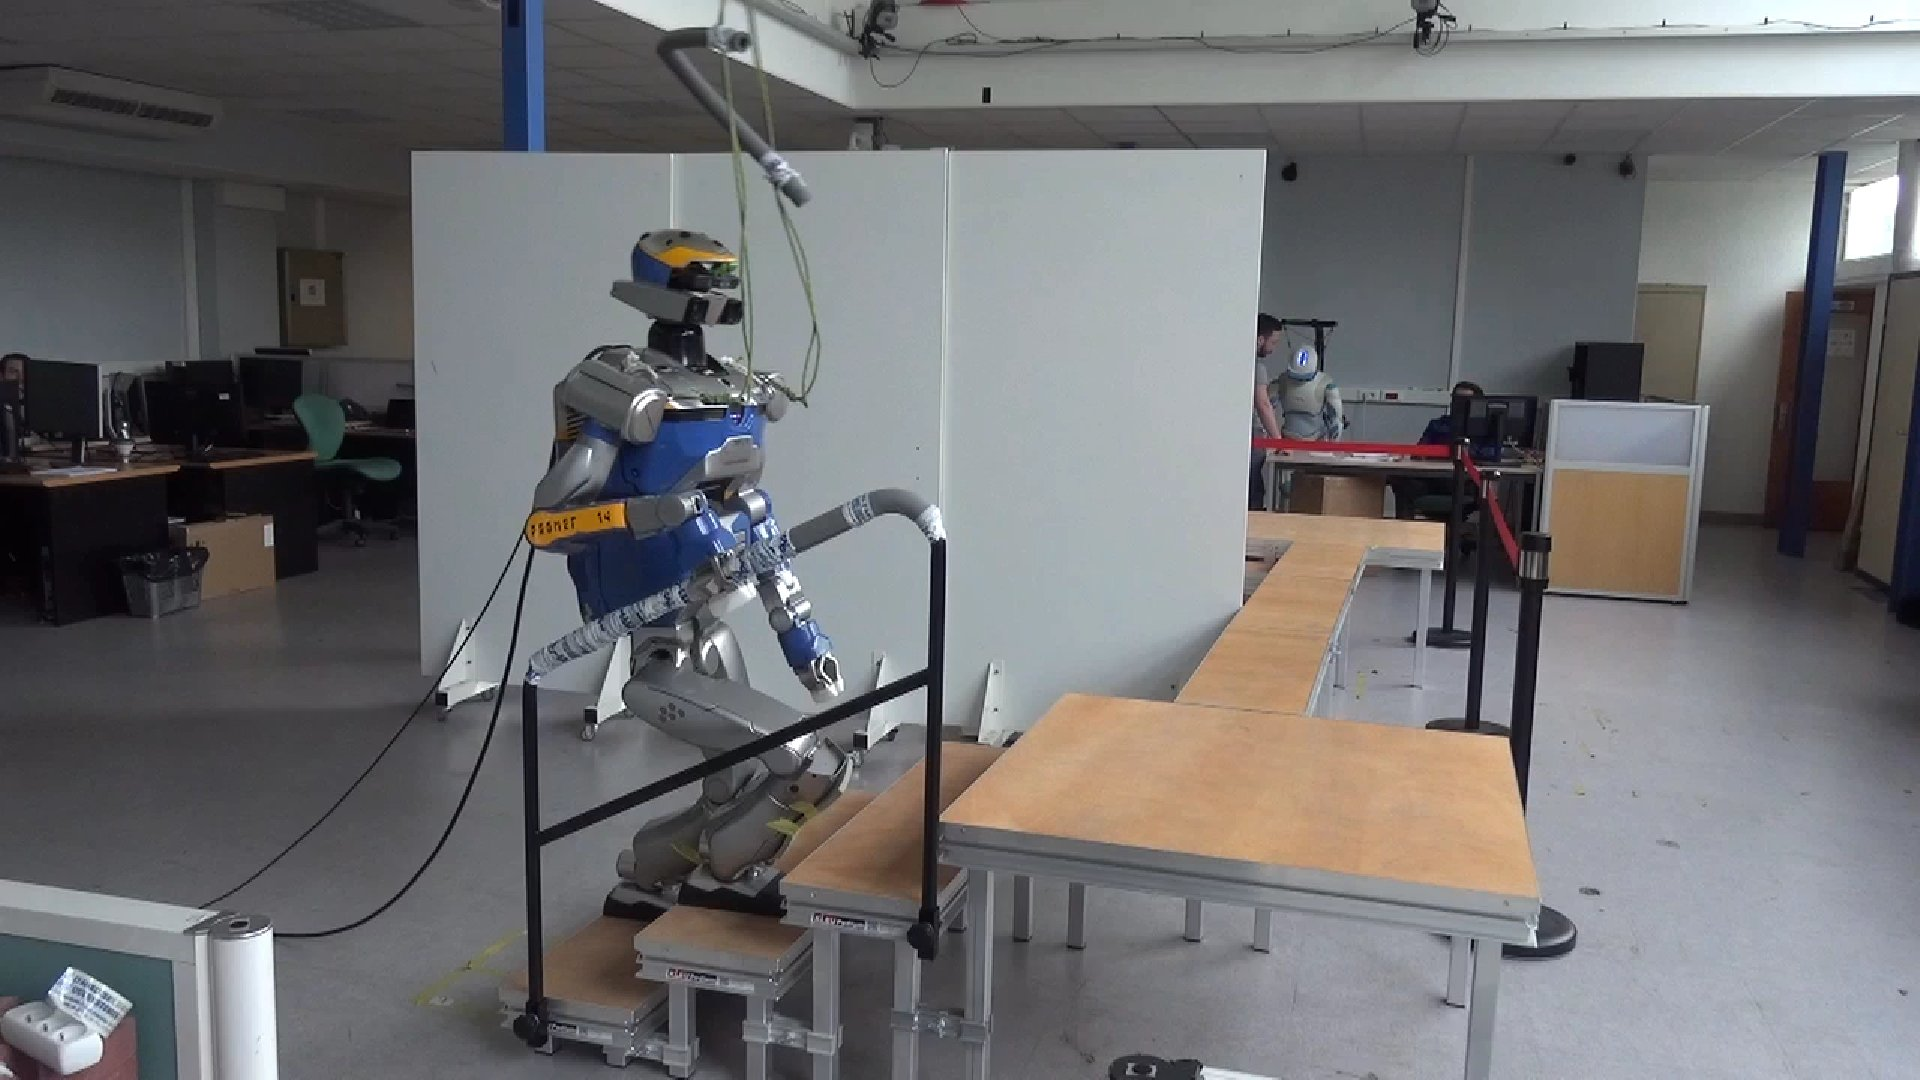
\includegraphics[trim={7.0cm 0.0cm 20.0cm 0.0cm}, clip, width=\widthValue]
    {./figures/stairclimbing4.jpeg}
  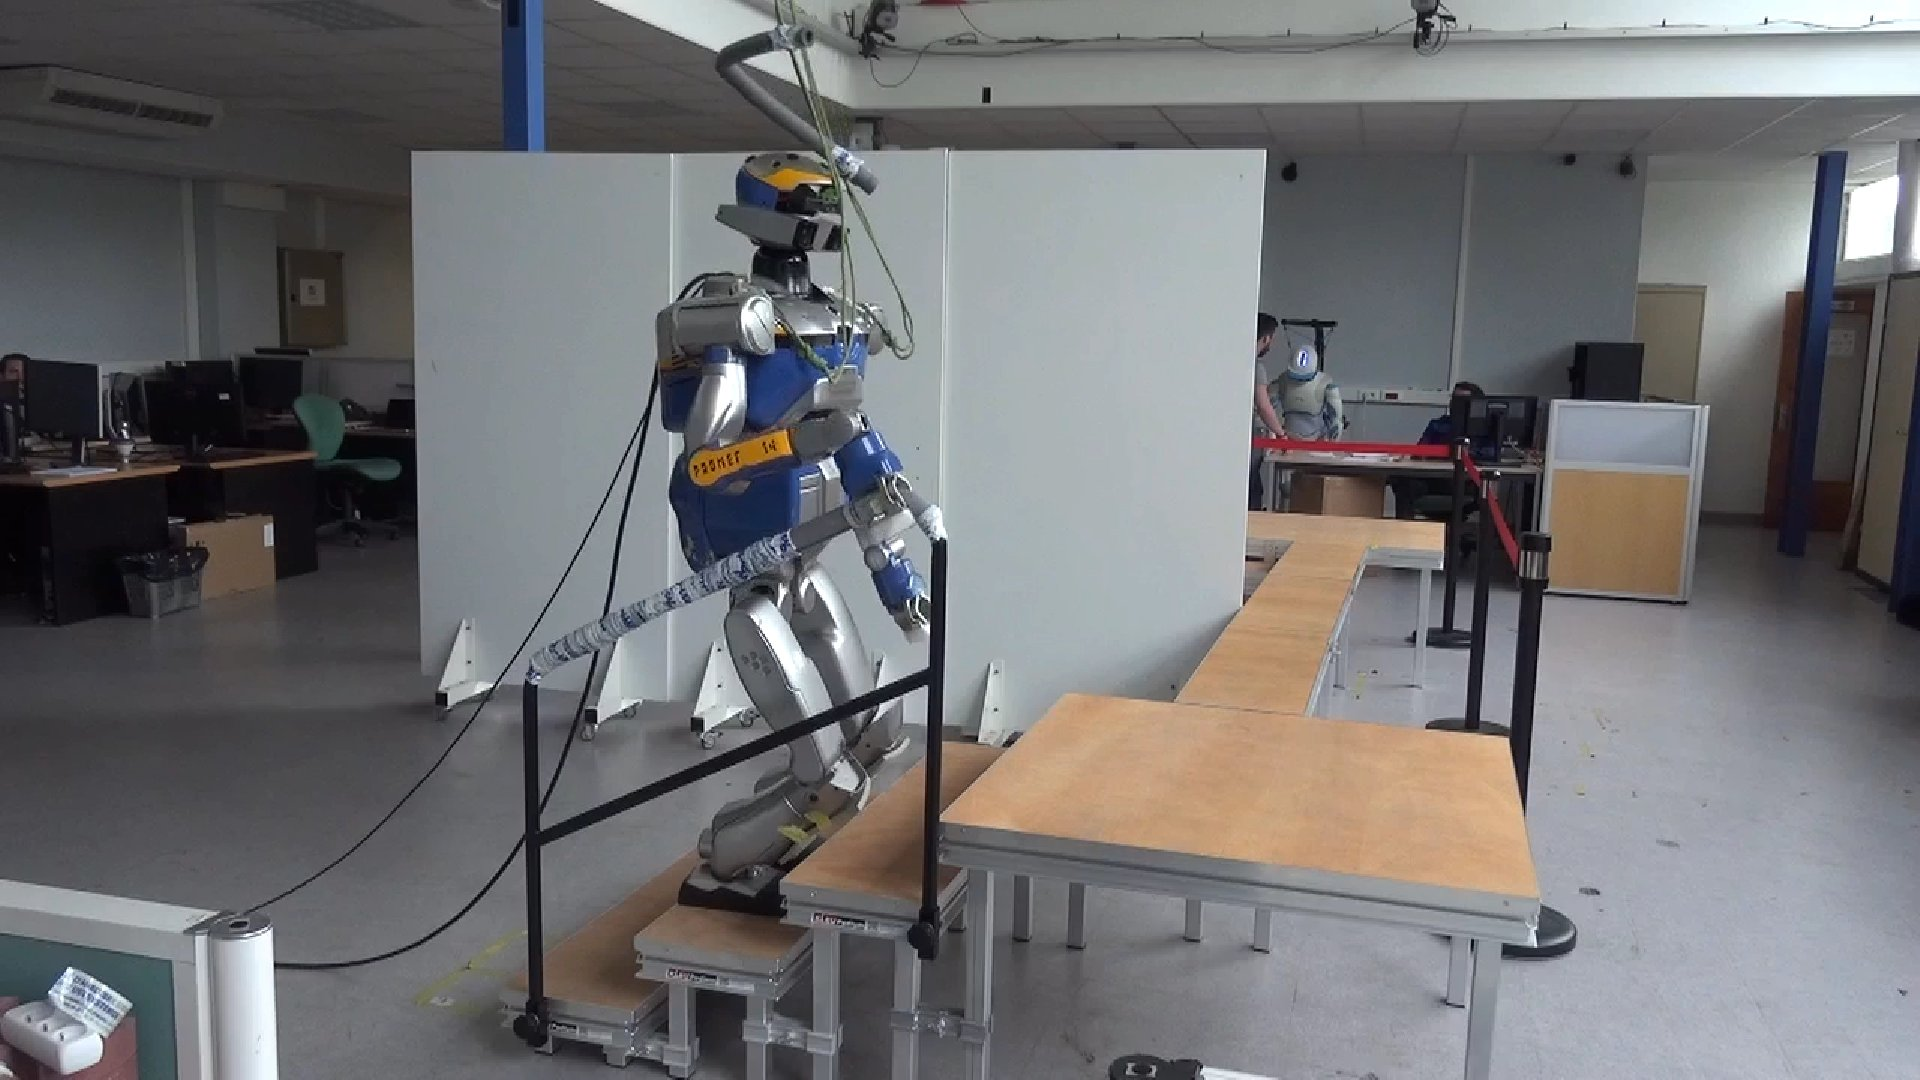
\includegraphics[trim={7.0cm 0.0cm 20.0cm 0.0cm}, clip, width=\widthValue]
    {./figures/stairclimbing5.jpeg}
  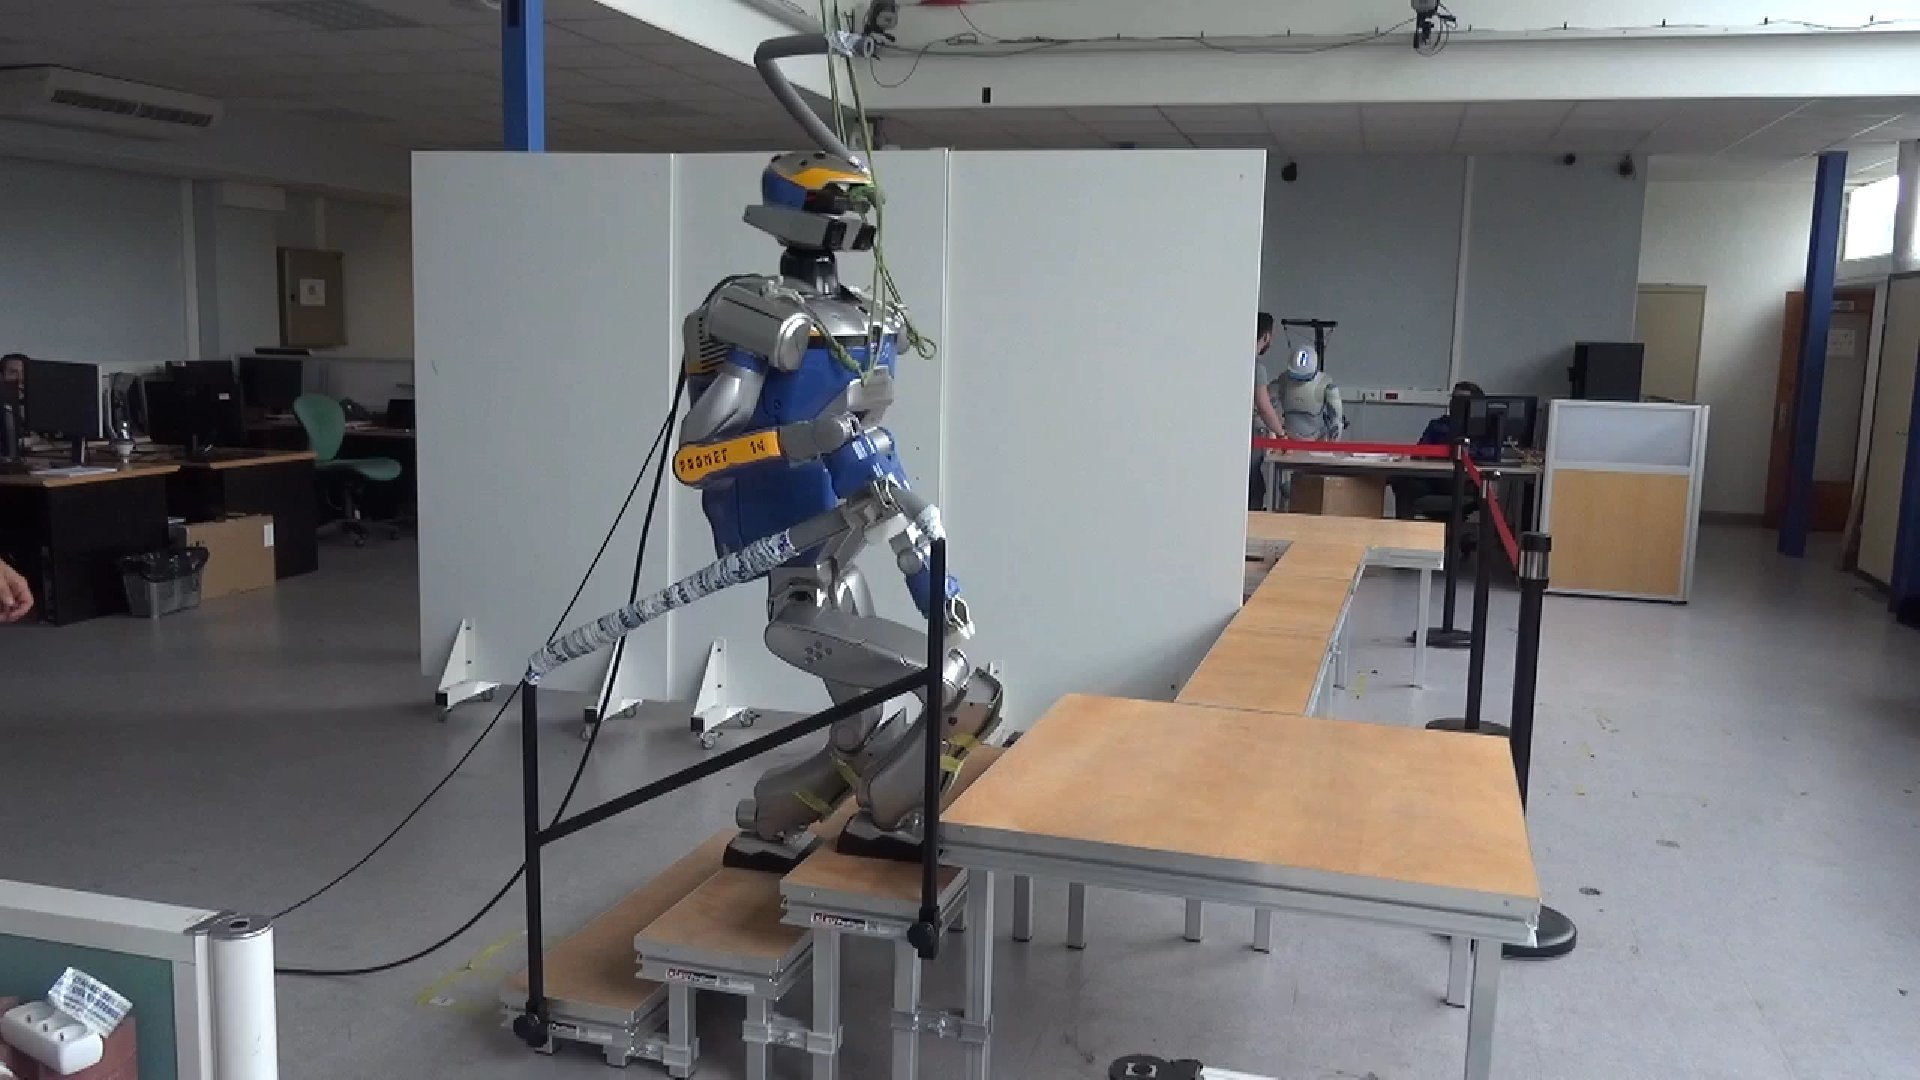
\includegraphics[trim={7.0cm 0.0cm 20.0cm 0.0cm}, clip, width=\widthValue]
    {./figures/stairclimbing6.jpeg}
  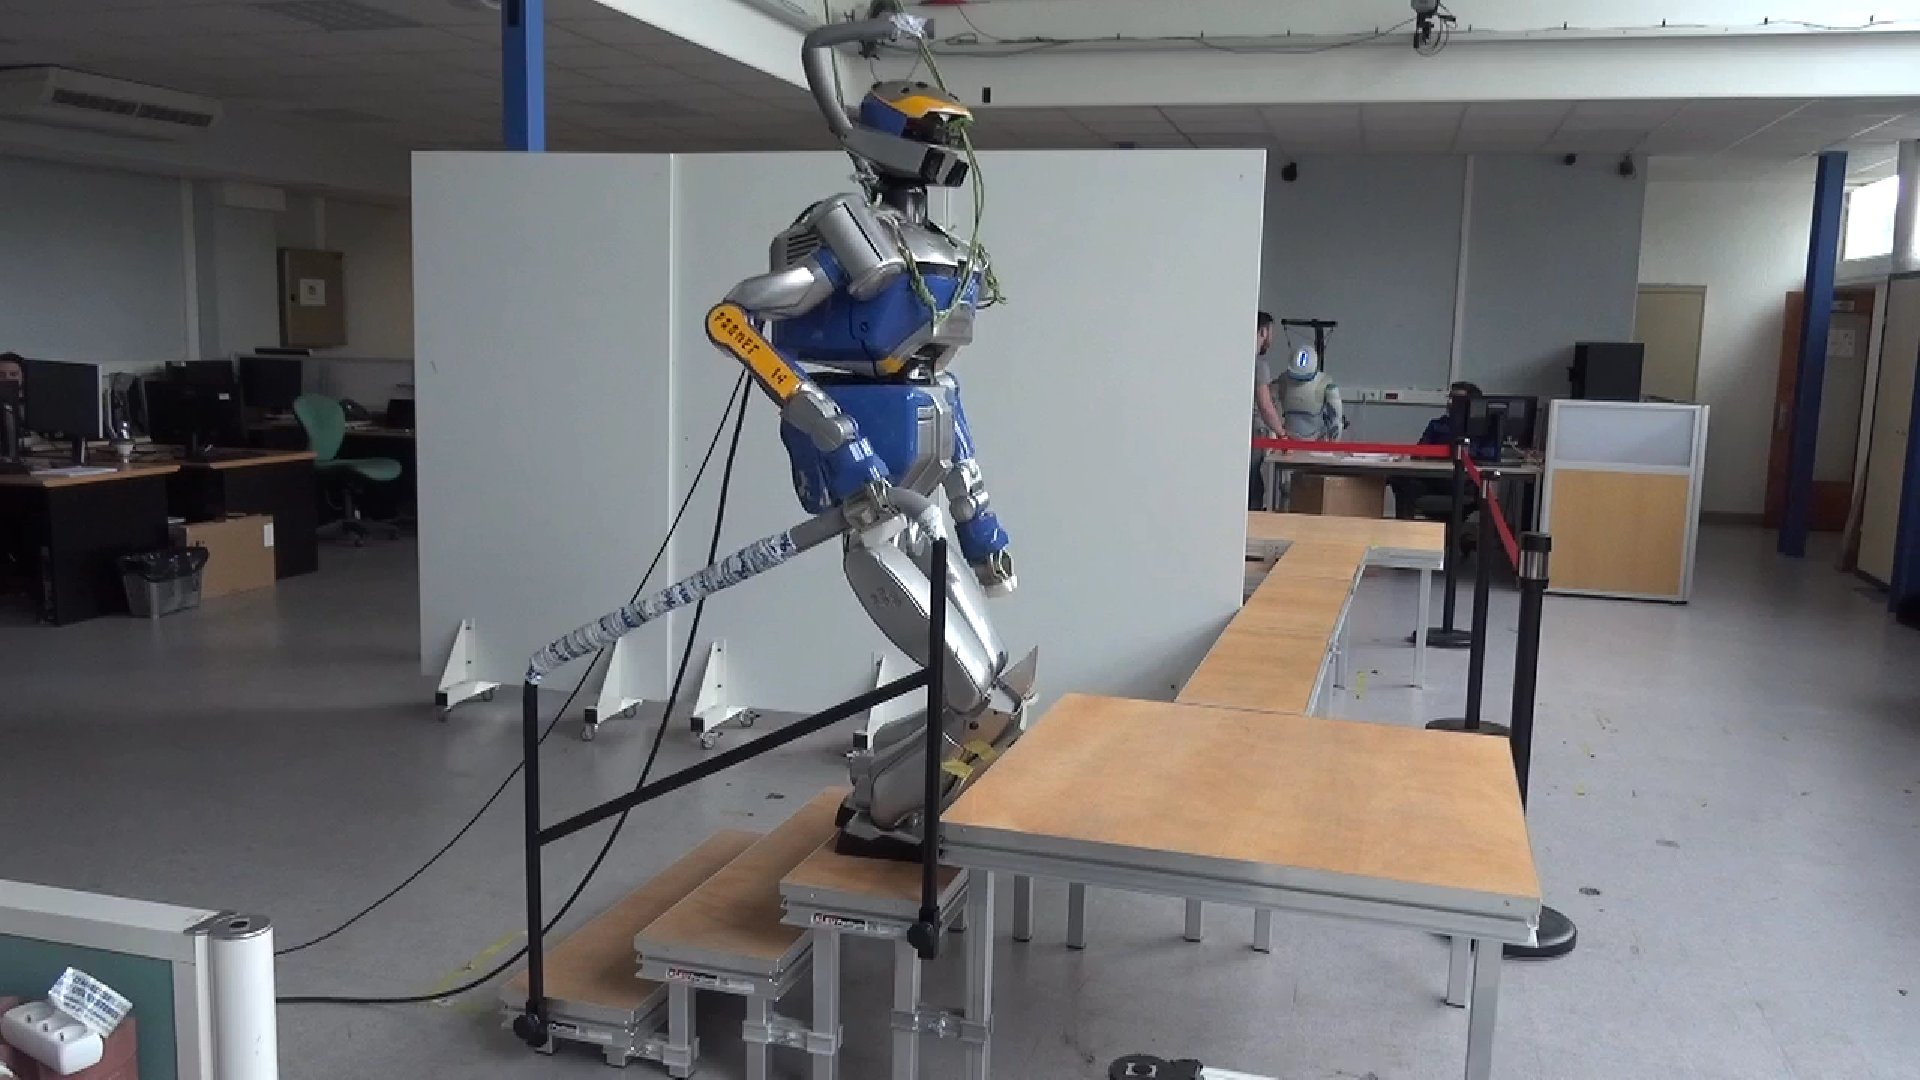
\includegraphics[trim={7.0cm 0.0cm 20.0cm 0.0cm}, clip, width=\widthValue]
    {./figures/stairclimbing7.jpeg}
  \caption{
           HRP-2 in the stair climbing scenario. }
		   \label{fig:stair_robust}
  \end{center}
  \vspace{-0.5cm}
\end{figure*}

The goal is to climb three 15-cm high steps.

\noindent\textbf{Contacts involved:} Feet and right arm.

\noindent\textbf{Heuristics:} The manipulability $h_w$ is chosen for the feet; $h_{\textrm{\it EFORT}}$ is chosen for the right arm.

\subsubsection{HyQ -- DRC-style rubble (Figure~\ref{fig:darpa})}
The quadruped robot must cross a rubble composed of bricks rotated at different angles and directions.

\begin{figure}
  \centering
  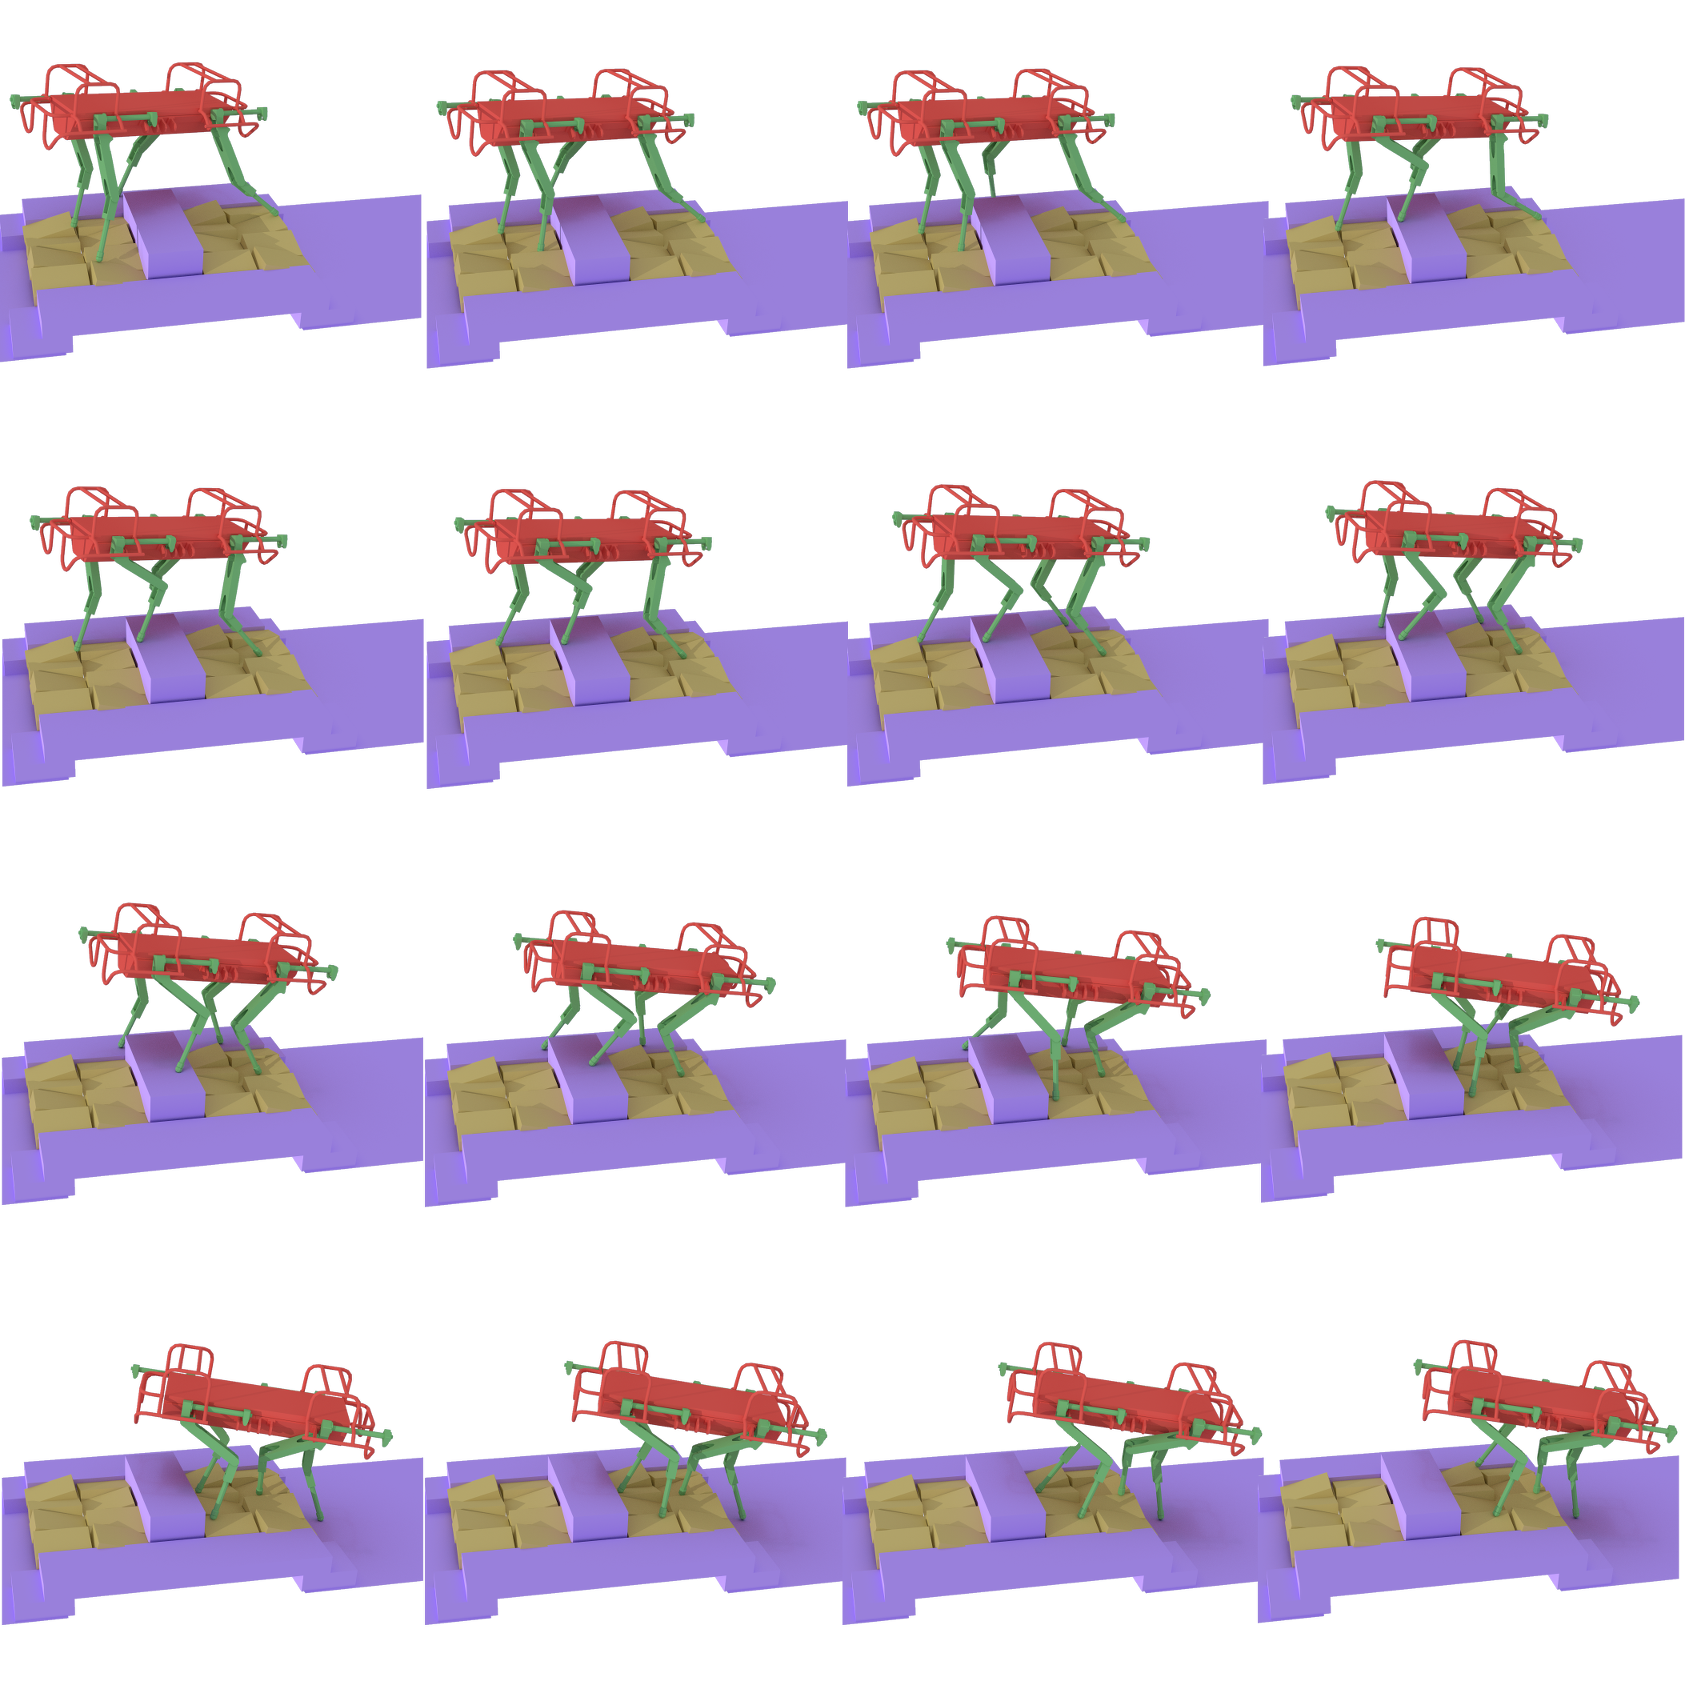
\includegraphics[width=1\linewidth]{figures/darpa}
  \caption{
           Robust crossing of rubbles by HyQ. }
		   \label{fig:darpa}
\end{figure}

\noindent\textbf{Contacts involved:} All (the 4 legs).

\noindent\textbf{Heuristics:} $h_w$. The robustness threshold $b_0$ is set to $20$.

\subsubsection{HyQ -- Obstacle race }
In this long scene, HyQ has to cross a 55-cm large hole, followed by a narrow ``bridge'', only 25-cm large.

\noindent\textbf{Contacts involved:} All (the 4 legs).

\noindent\textbf{Heuristics:} $h_w$. The robustness threshold $b_0$ is set to $10$.

\subsubsection{HRP-2 -- Path re-planning (Figure~\ref{fig:re-planning})}
In this long scene, HRP-2 plans a path through several obstacles. The scene is edited during the execution of the motion: a stair is added,
stepping stones are removed, as for parts of the final staircase. All these modifications require re-planning.

\begin{figure}
  \centering
  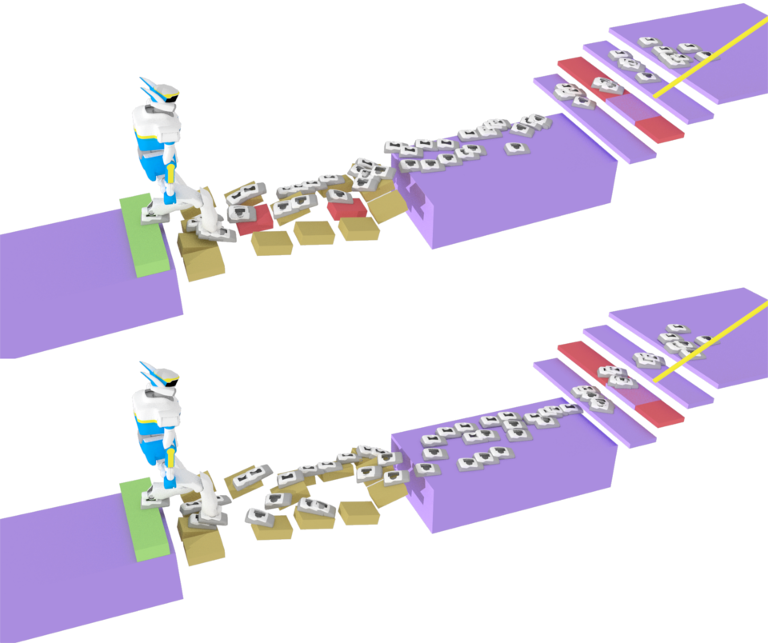
\includegraphics[width=0.7\linewidth]{figures/replanning}
  \caption{
           HRP-2 in the re-planning scenario. After the red step stones are removed, a new sequence of contacts is re-planned. Hand contacts
           are not presented here for readability.}
		   \label{fig:re-planning}
\end{figure}

\noindent\textbf{Contacts involved:} Feet and the right arm.

\noindent\textbf{Heuristics:} $h_w$  for all legs. $h_{\textrm{\it EFORT}}$  for the right arm. The robustness threshold is set to $2$.

\subsection{Role of the main parameters} \label{sec:influence}
We discuss the factors that influence the outcome of our planner: the root scaling factor $s$ (Section~\ref{sec:scaling}), the heuristics for
contact generation (Appendix~\ref{sec:heuristics}), and lastly, the discretization step for the guide path. The appropriate value for these parameters
is computed empirically based on use-case analysis or trials and errors.

\subsubsection{Choosing the scaling factor $s$} \label{sec:params}
For several values of $s$, we generated $10 000$ configurations. 
We then computed the sensitivity and specificity of the reachability condition.  In this context, the sensitivity refers to the percentage of configurations in $C_{Reach}^0$, effectively belonging to \gls{$C_{Contact}^0$}. If a sampled configuration is in $C_{Reach}^0$, but our method is unable to generate a contact configuration from it, as a result the sensitivity
decreases. The sensitivity thus illustrates the confidence we have that any configuration in $C_{Reach}^0$ will effectively lead to a contact configuration.
Conversely, the specificity refers to the percentage of configurations \textbf{not} in $C_{Reach}^0$, effectively \textbf{not} belonging to \gls{$C_{Contact}^0$}.
If a sampled configuration is \textbf{not} in $C_{Reach}^0$, but our method is able to generate a contact configuration from it, as a result the specificity
decreases. The specificity thus illustrates the confidence we have that all configurations that allow contact creation belong to $C_{Reach}^0$ (or informally, the confidence that we are not missing valid solutions).
We thus look for a compromise between sensitivity and specificity.

The obtained results for HRP-2 are shown in Table~\ref{tab:scale}, averaged over all scenes (except for the car egress: in this scenario, 
statistical tests are not really conclusive since we are only interested in a small area of the environment).

As it can be expected, the scaling results in a high increase of the sensitivity, with a decrease of the specificity.
For HRP-2 we decided to set $s^*=1.2$.

\begin{table}
\centering
\footnotesize
\begin{tabular}{c | c | c}
   Value of $s$ &  Sensitivity & Specificity\\
 \hline
   1   & 76\% & 100 \%\\
   1.1& 88\% & 96\% \\
   1.15& 93\% & 94\%\\
   1.2 & 97\% & 92.5\%\\
   1.25& 98\% & 91.7\%\\
   1.5 & 99\% & 90.5\%\\
 \end{tabular}
\caption{Sensitivity and specificity values of the reachability condition, depending on the scaling value $s$ of $W^0$.}
\label{tab:scale}
\quad
\end{table}

\subsubsection{Choosing the heuristics} \label{sec:heuristichoices}
In our conference paper~\citep{tonneauisrr15}, the computed motions were generated using the EFORT heuristic.
EFORT is designed for tasks requiring large magnitude contact forces (such as pushing / pulling / climbing). 
In locomotion tasks, such as the stair scenario, one issue with EFORT is that it tends to generate
configurations close to singularities (and joint limits). While this did not significantly impact
the generation of the plan, the resulting interpolation turned out to be harder.
For this reason, we use our manipulability-based heuristic for the legs, but still
use EFORT for the arms, which results in fewer contact repositionings.

\subsubsection{Discretization of the guide path} \label{sec:disc}
The discretization step is a user-defined, fixed parameter. The step
has an influence on the output of the planner: if too large steps are taken,
the planner may fail since we impose the constraint that only one contact change might occur
between two consecutive steps. On the other hand, a small step will not impact the success rate of the planner, 
but may generate unnecessary states. In most scenarios the torso of HRP-2 moves about 15 cm between two postures, but only 3 cm
for the car egress scenario to handle the geometry of the car.
For future work, we would like to automatically adapt the size of the discretization step.

\subsection{Performance analysis} \label{sec:perf}
To analyze performance, we ran the planner 1000 times for each scenario.
We measured the computation time spent in each part of the algorithm, and analyzed success rate.

\begin{table}
\centering
\begin{tabular}{ l | c}
  &  Path planning success rate \\
 \hline
   Stairs     	& 100\% \\
   Standing			& 68\% 	\\
   Car 			& 77\% 	\\
   Rubble 				& 97\% 	\\
   Race        & 88.0\% 	\\
 \end{tabular}
\caption{ Percentage of successful complete contact planning rates for each scenario, rounded to the first decimal.}
\label{tab:sucess_planning}
\quad
\end{table}

\begin{table}
\centering
\begin{tabular}{ l | >{\centering\arraybackslash}m{65pt} | >{\centering\arraybackslash}m{35pt} | >{\centering\arraybackslash}m{35pt} | c}
  &  Equilibrium success rate & Kinematic failure & Equilibrium failure \\
 \hline
   High stairs 	& 99.5\%  & 0.1\% 	& 0.4\% \\
   Standing up 		& 87.8\%  & 6.1\% 	& 6.1\% \\
   Car egress 		& 66.2\%  & 15.9\% 	& 17.9\% \\
   Rubble 			& 97.54\% & 0.16\% 	& 2.3\% \\
   Obstacle race 	& 92.4\%  & 0.15\% 	& 7.45\% \\
 \end{tabular}
\caption{Success rates obtained for the generation of static equilibrium contact configurations for each scenario, rounded to the first decimal. Column 1 indicates 
indicates the rate of contact generation that succeeded. In the cases where the generation fails, it can be
either a kinematic issue (column 2), or because no contact configuration led to a static equilibrium configuration (column 3). Note that a failure in the contact generation
is not equivalent to a failure of the contact planning algorithm.}
\label{tab:requestpercent}
\quad
\end{table}

\begin{table*}[b!t!p!]
\centering
\footnotesize
\begin{tabular}{ >{\centering\arraybackslash}m{37pt} | >{\centering\arraybackslash}m{57pt} | >{\centering\arraybackslash}m{65pt} | >{\centering\arraybackslash}m{70pt} | >{\centering\arraybackslash}m{73pt} | >{\centering\arraybackslash}m{80pt} | >{\centering\arraybackslash}m{10pt}}
  Scenario (nb steps) &  Complete guide generation (ms) & Static equilibrium (ms) & Collision (ms) & Inverse Kinematics (ms) & Total generation time (ms) & Time per step (ms)\\
 \hline
   Stairs (18) 	& 5 -- \textbf{6} --  18 		 & 13 --  \textbf{32} -- 329   	& 1 --  \textbf{4} -- 38 & 26 --  \textbf{127} -- 1345 & 92 --  \textbf{261} -- 2174 & \textbf{15} \\
   Standing (24)& 65 -- \textbf{1086} --  5227   & 27 --  \textbf{144} -- 338   & 2 --  \textbf{12} -- 37 & 144 --  \textbf{1046} -- 2374 & 371 --  \textbf{2257} -- 7671 & \textbf{94}  \\
   Car (86)& 320 -- \textbf{6971} --  44002 & 409 --  \textbf{1766} -- 14752   	& 297 -- \textbf{1187} -- 8483 & 3154 --  \textbf{15323} -- 165541 & 5834 --  \textbf{31391} -- 281000 & \textbf{365}\\
   Rubble (82)& 37 -- \textbf{573} --  1685 & 583 --  \textbf{2714} -- 9459 & 491 --  \textbf{1971} -- 6273 & 269 --  \textbf{706} -- 3118 & 1811 --  \textbf{7195} -- 23241 & \textbf{86} \\
   Race (134)& 14 -- \textbf{51} --  125 & 455 --  \textbf{1359} -- 21045   & 397 --  \textbf{923} -- 9924 & 228 --  \textbf{471} -- 5415 & 1436 --  \textbf{3343} -- 41446 & \textbf{25}
 \end{tabular}
\caption{minimum, \textbf{average} and worst time (in ms) spent in the generation process for each scenario and each critical part of the generation process (not all parts are timed,
thus the average total computation time is higher than the sum of each part). The last
column indicates the average time necessary to compute one contact transition. The Collision column times includes the (negligible) octree intersection operation necessary to retrieve the candidate samples.}
\label{tab:requestime}
\quad
\end{table*}

\subsubsection{Success rates (Table~\ref{tab:sucess_planning})}
Despite the complexity of the scenarios and the approximations made in our formulation, our planner succeeded in the large majority of cases.

Table~\ref{tab:requestpercent} presents the rate of successful contact generation. Note that a failure in contact generation for a root configuration is not equivalent to a failure in the contact plan. It simply means that another limb was tested for contact generation for the same root configuration.
As expected, a more constrained scenario such as the car egress provides less satisfying results, despite the high success rate of the planner.

\subsubsection{Computation times (Table~\ref{tab:requestime})}

For HRP-2, most of the time was spent performing inverse kinematics.
This is not surprising considering the number of calls to the methods: IK projection is used intensively to maintain contact continuity between two postures; 
it is also applied every time a new candidate needs to be evaluated. In particular for the car egress scenario,
the collision avoidance constraints are demanding.

On the other hand for HyQ most of the time is spent testing the static equilibrium of the candidate configurations.

In all scenarios, one can observe that the average computation time for one single step is largely below one second,
thus enabling \gls{interactive} applications and online autonomous planning of the robot motion.

\subsubsection*{Conclusion}
These results confirm that our approach provides a satisfying compromise between completeness and efficiency, thus enabling online planning
while controlling the robot. Indeed, when the contact planning fails, it fails rapidly. This allows us to rapidly re-plan with a reasonable chance of success.
The most efficient (and immediate) approach to obtain a valid contact plan as fast as possible would be to launch in parallel several instances of the planner (our current implementation is single-threaded) and to use any successful result as a plan for solver $\mathcal{P}_3$.

\begin{table}
\centering
\begin{tabular}{ c | c | c }
 Scenario & Method  & Computation time \\
 \hline
   \multirow{3}{*}{Stair 20 cm} & Hauser~\cite{Hauser06usingmotion} &  5.42 min  \\							 
							  & Mordatch et al.\cite{Mordatch:2012:DCB:2185520.2185539} & 2 to 10 min \\
							 & \textbf{Ours} + \cite{Carpentier2016}  & \textbf{$ <$ 2s} \\
 \hline
   \multirow{3}{*}{Stair 30 cm} & Hauser~\cite{Hauser06usingmotion} &  4.08 min  \\
							 & Mordatch et al.\cite{Mordatch:2012:DCB:2185520.2185539} & 2 to 10 min \\
							 & \textbf{Ours}  & \textbf{$ <$ 2s}   \\
 \hline
   \multirow{3}{*}{Stair 40 cm} & Hauser \cite{Hauser06usingmotion} &  10.08 min  \\
							 & Mordatch et al.\cite{Mordatch:2012:DCB:2185520.2185539} & 2 to 10 min \\
							 & \textbf{Ours}   & \textbf{$ <$ 5s}   \\
 \hline
   \multirow{2}{*}{Table (car) egress} & Bouyarmane et al.~\cite{Bouyarmane2009, DBLP:conf/iser/EscandeKMG08} & 3.5 hours  \\
							 & \textbf{Ours}  & \textbf{$<$ 60 s} \\

 \end{tabular}
\caption{Comparison between the computation times obtained by our method and previous ones for addressing the whole problem.}
\label{tab:compprev}
\quad
\end{table}

\subsection{Comparison with previous work} \label{sec:compa}
We did our best to provide a fair comparison of the computation complexity of our method with the state of the art. 
However existing benchmarks for motion planning algorithms~\cite{moll2014extensible} do not yet encompass contact planning.
Moreover, the source code of the previous methods of the state of the art is often not available.
Providing a fair comparison with the algorithms performing on the same computer and on the same scenarios is yet out of reach.
A step in this direction is the open-source release of our source code (see Section~\ref{app:hpp}) that allows any reader to reproduce our results.
Furthermore, $\mathcal{P}_3$ remains challenging in the presence of obstacles. The only valid scenarios addressed completely in previous works are thus the stair-climbing scenarios of different heights proposed by Hauser in \cite{Hauser06usingmotion}, and the table-egress scenario by Escande et al. in~\cite{DBLP:conf/iser/EscandeKMG08}, which we consider to be of similar complexity with respect to the car-egress scenario (we did not consider the stairs in the scene). Both scenarios are tested with HRP-2.

Table~\ref{tab:compprev} presents the computation times for these scenarios. Since no implementation of the previous methods is available, we had no choice but to indicate the times directly taken from their corresponding papers.
In the case of older contributions such as~\cite{Hauser06usingmotion},~\cite{DBLP:conf/iser/EscandeKMG08} and~\cite{Bouyarmane2009}, because of the technological progress, it appears that our results would have been more meaningful if the benchmarks were run on a modern computer. However, since the computation times differ of several orders of magnitude, we believe that these results clearly show the computational benefits of our method.

 \section{Discussion: validity and purpose of our contact planner} 
\label{sec:discussion}

As demonstrated in the results section, the main purpose of our method is the reduction of the algorithmic complexity of the problem, which leads to an interactive 
application. This property is critical for 
online applications with the robot and was not proposed by any of the previous contributions. Our method addresses highly constrained environments while improving the search time by orders of magnitude. This high performance is reached at the cost of some approximations that we discuss here. 

The first approximation is the verification of \contactreachability\ ($\mathbf{q}^0 \in C_{Contact}^0$).  Our \textit{reachability condition} ($\mathbf{q}^0 \in C_{Reach}^0$) is computationally efficient and provides an accurate approximation of $C_{Contact}^0$ (Section~\ref{sec:scaling}). This is demonstrated by the second column of Table~\ref{tab:requestpercent}, and illustrated by Figure~\ref{fig:dedefeas}. Indeed, in the large majority of cases, (84\% in the worst car egress case), we are able to find a contact configuration for any configuration in $C_{Reach}^0$.

Another source of computational cost identified in previous works is the verification of \equilibriumfeasibility. 
The main assumption of our work is that for the class of problems we consider \contactreachability\ implies \equilibriumfeasibility.
Our scenarios show that the  assumption is verified in the majority of cases when at least one contact surface is \textit{quasi flat}~\cite{Prete2016}, that is when
the friction cone of the contact surface contains the direction opposite to the gravity.
Figure~\ref{fig:dedefeas} illustrates this observation, demonstrated empirically by the third column of Table~\ref{tab:requestpercent}. In the worst case, in our experiment
the assumption was verified for 82\% of the total amount of trials that verified \textit{contact reachability}.
In the example of \cite{Bouyarmane2009}, the verification of \equilibriumfeasibility\ implies a constructive demonstration by exhibiting a valid $\mathbf{q}^{\overline{0}}$, requiring
several minutes of planning. Our method, in comparison, takes from a few milliseconds to several seconds.

These results clearly justify our pragmatic approach.

\begin{figure}[t]
\centering
  \begin{overpic}[width=1\linewidth]{figures/2D_feas}
		\put (15,) {$C_{Equil}^0$      $\subset$} 
		\put (47,) {$C_{Contact}^0$ $\approx$ } 
		\put (76,) {$C_{Reach}^0$} 
	\end{overpic}
\caption{Illustration of several root configurations sets used in this paper in a 2D scene. Obstacles are violet, and units are in meters. To show the sets in a 2D representation, all the rotational joints of HRP-2 are locked in the shown configuration, such that a torso configuration
is only described by two positional parameters (x and y). The root of the robot is indicated with a black cross. To compute the reachable workspace, the point on the ankle indicated by a green cross was used. $C_{Equil}^0$ is included in $C_{Contact}^0$. $C_{Reach}^0$ approximates $C_{Contact}^0$. Depending on a parametrization, we can obtain $C_{Contact}^0 \subset C_{Reach}^0$. Considering the configurations around the top obstacle, we can observe a similarity between  $C_{Equil}^0$  and $C_{Contact}^0$ when the reachable workspace of the legs includes \textit{quasi-flat} surfaces.}
		   \label{fig:dedefeas}
\end{figure}

\section{Conclusion} 
\label{sec:conclusion}

In this paper we consider the multi-contact planning problem, formulated as three sub-problems  $\mathcal{P}_1$,  $\mathcal{P}_2$,  $\mathcal{P}_3$, addressed sequentially. While we propose a global framework that handles all these problems, our contribution focuses on  $\mathcal{P}_1$ and  $\mathcal{P}_2$.
The first problem $\mathcal{P}_1$ consists in computing an \gls{equilibrium feasible} guide path for the root of the robot;
the second problem $\mathcal{P}_2$ is the computation of a discrete sequence of whole-body configurations along the root path.
We believe that this decomposition is currently the most promising approach towards
a global resolution of the problem. We also claim to have achieved a significant step towards this objective thanks to the dimensionality reduction provided by
the reachability condition. With our results and the release of our source code, we hope to inspire further research in this direction.

Our contribution to \Pa is the introduction of a low-dimensional space $C_{reach}^0$, an approximation of the space of \gls{equilibrium feasible} root configurations.
$C_{reach}^0$ can be efficiently sampled and has a low-dimension. For these reasons we are able to solve \Pa much faster than previous approaches.

Our contribution to \Pb is a fast contact generation scheme that can optimize user-defined criteria.

Our results demonstrate that our method allows a pragmatic compromise between three 
criteria that are hard to reconcile: generality, performance, and quality of the solution, making it the first acyclic contact
planner compatible with \gls{interactive} applications.

\textbf{Regarding generality}, the \textit{reachability condition}, coupled with an approach based on limb decomposition, 
allows the method to address automatically arbitrary legged robots.
\textbf{Regarding performance}, our framework is efficient in addressing both \Pa and $\mathcal{P}_2$. This results in \gls{interactive} computation times.
\textbf{Regarding the quality of the paths}, we are able to compute
\gls{equilibrium feasible} paths in all the presented scenarios, with high success rates.
As for \cite{Bouyarmane2009}, failures can still occur, due to the approximate condition used to compute the guide path.
The low computational burden of our framework however allows for fast re-planning in case of failure.
Furthermore, because of this approximation, the guide search is not complete. The choice is deliberate, because we believe
that it is necessary to trade completeness for efficiency at all stages of the planner.
However, one direction for future work is to focus on a more accurate formulation of $C_{reach}^0$ to improve
the approximation.

Our method applies to any scenario where at least one contact friction cone contains
the direction opposed to the gravity (i.e. \textit{quasi-flat}). This class of scenarios include all the problems proposed at the DARPA Robotics Challenge.
One way to further extend its range of application, which we consider for future work, is to include the equilibrium criterion when solving $\mathcal{P}_1$.
Considering the set of obstacles intersecting with the reachable workspace for a given root configuration as candidate surfaces, we can use them to verify the equilibrium criterion.
This would give us a necessary condition for \equilibriumfeasibility. %

While we have exhibited complete multi-contact locomotion obtained with our contact planner, our main concern for future work is to address the interpolation
between contact sequences ($\mathcal{P}_3$), which remains an open issue in highly-constrained scenarios.
Solving $\mathcal{P}_3$ requires addressing efficiently the collision avoidance problem in the interpolation phase, an issue 
not addressed by existing frameworks. We aim at providing our plans with transition certificates, that would define constraints on $\mathcal{P}_3$, under which
the transition between two contact configurations is feasible and collision-free.
Finally, we aim at performing kinodynamic planning to remove the constraint that configurations be in static equilibrium. We believe that the most promising direction in this regard is to integrate the notion of Admissible Velocity Propagation \citep{DBLP:conf/rss/PhamCN13}.
Addressing these two issues is essential to bridge the gap between the planning and control aspects of legged locomotion.

\appendices

\section{Generating the $W$ volumes for HRP-2}
\label{app:rom}

We detail our method to generate the volumes $W$ used
in RB-RRT, with the example of HRP-2.
The kinematic tree is split into four limbs $R^k$.
The arms are connected to the shoulders, and the legs to the root.
The obtained volumes $W$ are shown in Figure~\ref{fig:hrp2_w}.

\begin{figure}
\centering
  \begin{overpic}[width=1\linewidth]{figures/hrp2_w}
	\end{overpic}
\caption{The $W$ volumes computed for HRP-2. The red shapes are $W^0$. The green shapes represent the $W^k$.}
		   \label{fig:hrp2_w}
\end{figure}

\subsection{Step 1: computing the reachable workspace $W^k$ of a limb}

To generate a volume $W^k$, we proceed as follows:
\begin{enumerate}
\item Generate randomly $N$ valid limb configurations for $R^k$, for $N$ really large (say $100000$);
\item For each configuration, store the 3D position of the end effector joint relatively to the root of $R^k$; then compute the convex hull of the resulting point cloud;
\item The resulting polytope can contain a very large number of faces.  A last step is thus to simplify it using an incremental decimation method~\cite{Garland:1997:SSU:258734.258849}.
Variations of this method are commonly implemented in most authoring tools. For our experiments we used the blender decimate tool. Details of its use can be found in the static webpage associated with this paper (\url{http://stevetonneau.fr/files/publications/isrr15/tro_install.html\#decimate}). For HRP-2 we apply the operator with a ratio of $0.06$, resulting in a polytope of 38 faces for the arms and the legs.
\end{enumerate}

\begin{figure}
\centering
  \begin{overpic}[width=1\linewidth]{figures/roms}
	\end{overpic}
\caption{Different approximations of the range of motion of the right arm of HRP-2. Left: non convex-hull, computed with the powercrust algorithm~\citep{Amenta:2001:PC:376957.376986}. Middle:
convex hull of the reachable workspace. Right: Simplified hull used in our experiments.}
		   \label{fig:hrp2_roms}
\end{figure}

Figure~\ref{fig:hrp2_roms} illustrate the obtained $W^k$ for HRP-2.
Regarding the procedure, we can see that step 2 is conservative (Figure~\ref{fig:hrp2_roms}--right), which 
is acceptable, especially because the lost set essentially relates to configurations close to singularity (they are close to the boundaries of the reachable workspace, and
often not \gls{contact reachable}, as illustrated in Figure~\ref{fig:dedefeas}, where the exterior boundaries of the reachable workspace appear
red, thus not belonging to $C_{Contact}^0$). We choose again to be less complete but more efficient, regarding the number of collision tests to be performed by RB-RRT.
In step 1 on the other hand, selecting the convex hull (Figure~\ref{fig:hrp2_roms}--middle) instead of a minimum encompassing shape (Figure~\ref{fig:hrp2_roms}--left) may introduce false positives.
Concretely, because the false positive set intersects with $W^0$, the scaling volume of the robot torso, the induced error is compensated,
as verified by the results shown by Table~\ref{tab:requestpercent}.

\subsection{Step 2: computing the torso scaling workspace $W^0$}
To define the volume $W^0$ of HRP-2, we proceed in an empirical manner.
First, we compute the bounding boxes of the robot torso, head, and upper legs (Figure~\ref{fig:hrp2_w} -- red shapes).
Then, we perform a scaling of these boxes by a factor $s$. 
The higher $s$ is, the more likely sampled configurations are to be feasible, but the less complete is the approach.
To compute the appropriate value of $s$, we proceed as described in Section~\ref{sec:params}, and choose empirically
$s^*=1.2$ as the appropriate value for HRP-2.
\section{Manipulability-based heuristics for contact selection}
\label{sec:heuristics}
This Section proposes two heuristics to select a contact that optimizes desired capabilities.
For instance, one can be interested in configurations that allow to efficiently exert a force in the global direction of motion, or to stay away from singular configurations.
We derive these heuristics from the work by \cite{Yoshikawa1984}, recalled here. %

\subsubsection{The force and velocity ellipsoids}

We consider: a limb configuration $\mathbf{q}^k$; its end effector position $\mathbf{p}^k$; its Jacobian matrix
$\mathbf{J}^k(\mathbf{q}^k)$; a force $\mathbf{f}$ exerted by the end effector. For clarity in the rest of the section we omit the $k$ indices and write $\mathbf{J}^k(\mathbf{q}^k)$ as $\mathbf{J}$.
Yoshikawa~\cite{Yoshikawa1984} defines the velocity (\ref{eq:vel}) and force~(\ref{eq:for}) ellipsoids:

 \begin{equation} 
 \label{eq:vel}
\mathbf{\dot{p}}^T(\mathbf{J}\mathbf{J}^T)^{-1}\mathbf{\dot{p}} \leq 1 
\end{equation}

 \begin{equation} 
 \label{eq:for}
\mathbf{f}^T (\mathbf{J}\mathbf{J}^T) \mathbf{f} \leq 1
\end{equation}

They describe the set of end-effector velocities (respectively forces) that can
be reached under the constraint $||\dot{\mathbf{q}}||^2 \leq 1$ for the current configuration.
The longer the axis of the ellipsoid is, the more important the velocity (resp. force) of the end-effector the direction of the axis can be.

\subsubsection{Manipulability-based heuristics}
From these definitions, we derive two heuristics that account for the environment and the task being performed.
The first one, EFORT, was introduced by \cite{Tonneau2014}; the second one derives the manipulability measure proposed by Yoshikawa~\cite{Yoshikawa1984}.

With EFORT, we define the efficiency of a configuration as the ability of a limb to exert a force in a given direction.
In a given direction $\uprho$, the length of the ellipsoid is given by the force-transmission ratio \citep{1087795}:
\begin{equation*}
f_\mathsf{T}(\mathbf{q}, \uprho) = [\uprho^{T}(\mathbf{J}\mathbf{J}	^{T})\uprho]^{-\frac{1}{2}}
\end{equation*}

To compare candidate configurations, we include the quality of the contact surface, and choose $\uprho$ as the direction opposite to the local motion (given by the difference between two consecutive root positions):

\begin{equation}
h_{\textrm{\it EFORT}}(\mathbf{q}, \uprho) = [\uprho^{T}(\mathbf{J}\mathbf{J}^T)\uprho]^{-\frac{1}{2}} ( \mu \mathbf{n}^T \uprho)
\end{equation}
where $\mu$ and $\mathbf{n}$ are respectively the friction coefficient and the normal vector of the contact surface.

$h_{\textrm{\it EFORT}}$ will favor contacts that allow large efforts. Alternatively, the manipulability measure can be considered~\cite{Yoshikawa1984}:

\begin{equation} \label{ellipsoid}
h_{w}(\mathbf{q}) = \sqrt{det(\mathbf{J}\mathbf{J}^T)}
\end{equation}

\section{Addressing $\mathcal{P}_3$}
\label{app:optim}
The stair climbing and the standing up scenarios were validated with the trajectory optimization scheme provided in \citeauthor{Carpentier2016}. 
To address the other scenarios, we propose a new implementation, entirely open source (\url{http://stevetonneau.fr/files/publications/isrr15/tro_install.html\#optim} ), which can be integrated directly in our motion planner software. This formulation uses the center of mass acceleration and angular momentum as input variables, while previously the contact forces were used.
The obtained COM trajectory is then turned into a collision-free whole-body trajectory.

We rewrite Eq.~\ref{eq:new_eul} in the general case:

\begin{align} \label{eq:new_eul_acc}
\mathbf{G} \bm{\beta} = 
\underbrace{\mat{m (\mathbf{\ddot{c}} - \mathbf{g}) \\m \mathbf{c} \times (\mathbf{\ddot{c}} - \mathbf{g}) + \dot{L}}}_{\mathbf{w}}
\end{align}

\noindent where $\dot{L}$ is the angular momentum expressed at the com.
Eq.~\ref{eq:new_eul_acc} defines a 6-dimensional cone $\mathcal{K}$ ~\citep{qiu:dhm:2011,Caron2015}. For a given set of contacts,
this cone determines all the admissible wrenches $\mathbf{w}$ that can be generated by contact forces inside their friction cones.
The face form of $\mathcal{K}$ can be computed using the double description method~\citep{Fukuda1996}:

\begin{equation}
\label{eq:cone_k}
	\mathcal{K} =  \left\{ \mathbf{w}, \mathbf{A}\mathbf{w} \leq \mathbf{b	} \right\}
\end{equation}

The objective 
is then to plan a trajectory for the center of mass such that the generated $\mathbf{w}$ always verifies Eq.~\ref{eq:cone_k}. 
We now consider two contact configurations  $\mathbf{q}_0$ and $\mathbf{q}_1$ computed by our planner: in the general case one contact is broken and one created to get from
$\mathbf{q}_0$ to $\mathbf{q}_1$. We manually define the duration of each of the three contact phases.
In each phase $s$ the centroidal wrench $\mathbf{w}$ is constrained to lie inside a cone $\mathcal{K}_u, u =0 \dots 2$.
We call the total duration of the motion $T$, and formulate the following optimization problem:

\begin{equation} \label{eq:qp_rob} \begin{aligned}
\minimize_{\mathbf{\ddot{c}}(t), \dot{L}(t)}  \quad & \sum_{u=0}^{2} \int_{t_u}^{t_u + \Delta t_u}  \ell(\mathbf{\ddot{c}}(t), \dot{L}(t)) \text{dt}  \\
\st \quad & \mathbf{A}_u \mathbf{w}(t)  \leq \mathbf{b}_u , \forall t \in  \left[t_u, t_u + \Delta t_u \right[, \forall u \\
	\quad & \mathbf{Y}_u \mathbf{c}(t)  \leq \mathbf{y}_u , \forall t \in  \left[t_u, t_u + \Delta t_u \right[, \forall u \\
	\quad & \mathbf{c}(0)  = \mathbf{c}_{\mathbf{q}_0} \\
	\quad & \mathbf{c}(T)  = \mathbf{c}_{\mathbf{q}_1} \\
	\quad & \mathbf{c}(0)  = \mathbf{\dot{c}}(0)  = \mathbf{\ddot{c}}(0) = \mathbf{0}\\
	\quad & \mathbf{c}(T)  = \mathbf{\dot{c}}(T)  = \mathbf{\ddot{c}}(T) = \mathbf{0}\\
\end{aligned} \end{equation}
The cost function $\ell$ is a weighted sum of the angular momentum and center-of-mass acceleration variation over the whole trajectory.
The center-of-mass positions and velocities $\mathbf{c}(t)$, $\mathbf{\dot{c}}(t)$ are internal variables, obtained through the double integration of $\mathbf{\ddot{c}}(t)$.
Then $\mathbf{w}(t)$ is obtained directly from these variables. $\mathbf{c}_{\mathbf{q}_0}$ and $\mathbf{c}_{\mathbf{q}_1}$ are the center-of-mass positions for configurations
 $\mathbf{q}_0$ and $\mathbf{q}_1$ respectively.
$\mathbf{Y}_u$ and $\mathbf{y}_u$ denote stacked kinematic constraints on the center of mass position, determined by the active contact locations.
The inequalities for each contact are determined in the same way that the reachable workspace is computed in Appendix~\ref{app:rom}, with
the effector serving as root. %

This formulation can trivially be extended over the whole contact sequence.
In our implementation, the problem is discretized using time steps of 100 ms. 

The output of this optimization problem is an admissible center-of-mass trajectory.
To compute the whole body motion, we use a two-step approach.

First, we plan a kinematic motion for the robot, subject to the contact constraints. We also constrain the center of mass to follow
the computed trajectory. This is achieved using a constraint-based RRT planner~\citep{7759083}. As a result we obtain a collision-free whole-body motion.

The entire resolution takes approximatively 1.5 seconds for a complete contact transition.

\section*{Acknowledgements}
This research is supported by Euroc (project under FP7 Grant Agreement  608849);  Entracte (ANR  grant  agreement  13-CORD-002-01);
the ARO Contract W911NF-14-1-0437; and the NSF award 1305286. %

\bibliographystyle{IEEEtran}
\bibliography{biblio}

\begin{IEEEbiography}[{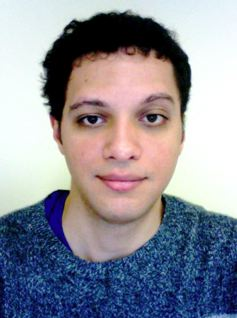
\includegraphics[width=1in,height=1.25in,clip,keepaspectratio]{figures/bio/steve}}]{Steve Tonneau} is a post-doctorate in the Gepetto team at LAAS-CNRS. He received the joint M.Eng. and M.Sc. degrees from Insa Rennes in 2008. After 4 years in the industry he defended his Phd in 2015 at the INRIA/IRISA Mimetic research team. His research focuses on motion planning based for legged avatars in arbitrary situations. Applications include computer graphics animation and legged robotics.
\end{IEEEbiography}

\begin{IEEEbiography}[{
\includegraphics[width=1in,height=1.25in,clip,keepaspectratio]{figures/bio/andrea}}]{Andrea Del Prete} received his degree in Computer
Engineering (with honors) from the 2nd faculty of
the University of Bologna (Italy) in 2009. In March
2013 he got his PhD from the Cognitive Humanoids
laboratory, Italian Institute of Technology, Genova
(Italy). From 2014 to 2017 he had been a PostDoc
at LAAS-CNRS in Toulouse (France), working on
optimization-based control of the humanoid robot
HRP-2. Since 2018 he is a senior researcher at
the Max Planck Institute for Intelligent Systems, in
Tuebingen (Germany).
\end{IEEEbiography}

\begin{IEEEbiography}[{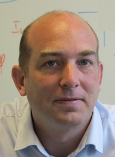
\includegraphics[width=1in,height=1.25in,clip,keepaspectratio]{figures/bio/julien}}]{Julien Pettré}
is a computer scientist. He is junior researcher at Inria, the French National Institute for Research in Computer Science and Control, in the Lagadic team. He received PhD from the University of Toulouse III in 2003, and Habilitation from the University of Rennes I in 2015. From 2004 to 2006, he was postdoctoral fellow at EPFL in Switzerland. He joined Inria in 2006.
Julien Pettré is currently coordinator of the European H2020 Crowdbot project (2018-21), dedicated to the design of robot navigation techniques for crowded environments. He previously coordinated the national ANR JCJC Percolation project (2013-17) dedicated to the design of new microscopic crowd simulation algorithms, as well as the national ANR CONTINT Chrome project, dedicated to efficient and designer-friendly techniques for crowd animation.
His research interests are crowd simulation, computer animation, virtual reality, robot navigation and motion planning. 
\end{IEEEbiography}

\begin{IEEEbiography}[{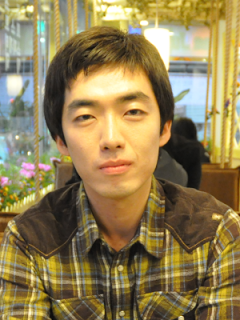
\includegraphics[width=1in,height=1.25in,clip,keepaspectratio]{figures/bio/chonhyon}}]{Chonhyon Park}
received the B.S. degree and the M.S. degree in computer science and engineering from the Seoul National University, Seoul, South Korea 2005 and 2007, respectively.

He received the Ph.D. degree in computer science at University of North Carolina at Chapel Hill in 2016.

His current research interests include motion and path planning,  navigation of virtual characters, and many-core computing.
\end{IEEEbiography}

\begin{IEEEbiography}[{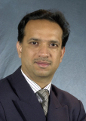
\includegraphics[width=1in,height=1.25in,clip,keepaspectratio]{figures/bio/dinesh}}]{Dinesh Manocha}
is currently the Phi Delta
Theta/Mason Distinguished Professor of Computer
Science at the University of North Carolina at
Chapel Hill. He received his Ph.D. in Computer
Science at the University of California at Berkeley
1992. Along with his students, Manocha has
also received 15 best paper awards at the leading
conferences. He has published more than 480
papers and some of the software systems related
to collision detection, GPU-based algorithms and
geometric computing developed by his group have
been downloaded by more than 200,000 users and are widely used in the
industry. He has supervised 33 Ph.D. dissertations and is a fellow of ACM, AAAI,
AAAS, and IEEE. He received Distinguished Alumni Award from Indian
Institute of Technology, Delhi.
\end{IEEEbiography}

\begin{IEEEbiography}[{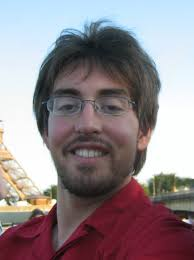
\includegraphics[width=1in,height=1.25in,clip,keepaspectratio]{figures/bio/nicolas}}]{Nicolas Mansard}
received the joint M.Eng. and
M.Sc. degrees in 2003, robotics and image process-
ing from Nationale Supérieure d'Informatique et de
Mathématiques Appliquées de Grenoble,
France, and University Joseph Fourier, Grenoble,
France, respectively, and the Ph.D. degree in robotics
for his work with Lagadic Group, Institut National
de Recherche en Informatique et en Automatique,
Rennes, France, in 2006. He spent one year with
Stanford University, Stanford, CA, with O. Khatib
and one year with JRL-Japan with A. Kheddar. He
is currently with the GEPETTO Group, LAAS- CNRS, Toulouse, France.
He was an Invited Researcher with Emo Todorovs Group, University of
Washington, in 2013. His research interest includes the generation of dynamic
sensor-based robot movements. Dr. N. Mansard received the CNRS Bronze
medal in 2015.
\end{IEEEbiography}

\end{document}
